% Options for packages loaded elsewhere
\PassOptionsToPackage{unicode}{hyperref}
\PassOptionsToPackage{hyphens}{url}
\PassOptionsToPackage{dvipsnames,svgnames,x11names}{xcolor}
%
\documentclass[
]{article}

\usepackage{amsmath,amssymb}
\usepackage{iftex}
\ifPDFTeX
  \usepackage[T1]{fontenc}
  \usepackage[utf8]{inputenc}
  \usepackage{textcomp} % provide euro and other symbols
\else % if luatex or xetex
  \usepackage{unicode-math}
  \defaultfontfeatures{Scale=MatchLowercase}
  \defaultfontfeatures[\rmfamily]{Ligatures=TeX,Scale=1}
\fi
\usepackage{lmodern}
\ifPDFTeX\else  
    % xetex/luatex font selection
\fi
% Use upquote if available, for straight quotes in verbatim environments
\IfFileExists{upquote.sty}{\usepackage{upquote}}{}
\IfFileExists{microtype.sty}{% use microtype if available
  \usepackage[]{microtype}
  \UseMicrotypeSet[protrusion]{basicmath} % disable protrusion for tt fonts
}{}
\makeatletter
\@ifundefined{KOMAClassName}{% if non-KOMA class
  \IfFileExists{parskip.sty}{%
    \usepackage{parskip}
  }{% else
    \setlength{\parindent}{0pt}
    \setlength{\parskip}{6pt plus 2pt minus 1pt}}
}{% if KOMA class
  \KOMAoptions{parskip=half}}
\makeatother
\usepackage{xcolor}
\usepackage[top=30mm,left=20mm]{geometry}
\setlength{\emergencystretch}{3em} % prevent overfull lines
\setcounter{secnumdepth}{5}
% Make \paragraph and \subparagraph free-standing
\makeatletter
\ifx\paragraph\undefined\else
  \let\oldparagraph\paragraph
  \renewcommand{\paragraph}{
    \@ifstar
      \xxxParagraphStar
      \xxxParagraphNoStar
  }
  \newcommand{\xxxParagraphStar}[1]{\oldparagraph*{#1}\mbox{}}
  \newcommand{\xxxParagraphNoStar}[1]{\oldparagraph{#1}\mbox{}}
\fi
\ifx\subparagraph\undefined\else
  \let\oldsubparagraph\subparagraph
  \renewcommand{\subparagraph}{
    \@ifstar
      \xxxSubParagraphStar
      \xxxSubParagraphNoStar
  }
  \newcommand{\xxxSubParagraphStar}[1]{\oldsubparagraph*{#1}\mbox{}}
  \newcommand{\xxxSubParagraphNoStar}[1]{\oldsubparagraph{#1}\mbox{}}
\fi
\makeatother


\providecommand{\tightlist}{%
  \setlength{\itemsep}{0pt}\setlength{\parskip}{0pt}}\usepackage{longtable,booktabs,array}
\usepackage{calc} % for calculating minipage widths
% Correct order of tables after \paragraph or \subparagraph
\usepackage{etoolbox}
\makeatletter
\patchcmd\longtable{\par}{\if@noskipsec\mbox{}\fi\par}{}{}
\makeatother
% Allow footnotes in longtable head/foot
\IfFileExists{footnotehyper.sty}{\usepackage{footnotehyper}}{\usepackage{footnote}}
\makesavenoteenv{longtable}
\usepackage{graphicx}
\makeatletter
\def\maxwidth{\ifdim\Gin@nat@width>\linewidth\linewidth\else\Gin@nat@width\fi}
\def\maxheight{\ifdim\Gin@nat@height>\textheight\textheight\else\Gin@nat@height\fi}
\makeatother
% Scale images if necessary, so that they will not overflow the page
% margins by default, and it is still possible to overwrite the defaults
% using explicit options in \includegraphics[width, height, ...]{}
\setkeys{Gin}{width=\maxwidth,height=\maxheight,keepaspectratio}
% Set default figure placement to htbp
\makeatletter
\def\fps@figure{htbp}
\makeatother
% definitions for citeproc citations
\NewDocumentCommand\citeproctext{}{}
\NewDocumentCommand\citeproc{mm}{%
  \begingroup\def\citeproctext{#2}\cite{#1}\endgroup}
\makeatletter
 % allow citations to break across lines
 \let\@cite@ofmt\@firstofone
 % avoid brackets around text for \cite:
 \def\@biblabel#1{}
 \def\@cite#1#2{{#1\if@tempswa , #2\fi}}
\makeatother
\newlength{\cslhangindent}
\setlength{\cslhangindent}{1.5em}
\newlength{\csllabelwidth}
\setlength{\csllabelwidth}{3em}
\newenvironment{CSLReferences}[2] % #1 hanging-indent, #2 entry-spacing
 {\begin{list}{}{%
  \setlength{\itemindent}{0pt}
  \setlength{\leftmargin}{0pt}
  \setlength{\parsep}{0pt}
  % turn on hanging indent if param 1 is 1
  \ifodd #1
   \setlength{\leftmargin}{\cslhangindent}
   \setlength{\itemindent}{-1\cslhangindent}
  \fi
  % set entry spacing
  \setlength{\itemsep}{#2\baselineskip}}}
 {\end{list}}
\usepackage{calc}
\newcommand{\CSLBlock}[1]{\hfill\break\parbox[t]{\linewidth}{\strut\ignorespaces#1\strut}}
\newcommand{\CSLLeftMargin}[1]{\parbox[t]{\csllabelwidth}{\strut#1\strut}}
\newcommand{\CSLRightInline}[1]{\parbox[t]{\linewidth - \csllabelwidth}{\strut#1\strut}}
\newcommand{\CSLIndent}[1]{\hspace{\cslhangindent}#1}

\usepackage[noblocks]{authblk}
\renewcommand*{\Authsep}{, }
\renewcommand*{\Authand}{, }
\renewcommand*{\Authands}{, }
\renewcommand\Affilfont{\small}
\makeatletter
\@ifpackageloaded{caption}{}{\usepackage{caption}}
\AtBeginDocument{%
\ifdefined\contentsname
  \renewcommand*\contentsname{Table of contents}
\else
  \newcommand\contentsname{Table of contents}
\fi
\ifdefined\listfigurename
  \renewcommand*\listfigurename{List of Figures}
\else
  \newcommand\listfigurename{List of Figures}
\fi
\ifdefined\listtablename
  \renewcommand*\listtablename{List of Tables}
\else
  \newcommand\listtablename{List of Tables}
\fi
\ifdefined\figurename
  \renewcommand*\figurename{Figure}
\else
  \newcommand\figurename{Figure}
\fi
\ifdefined\tablename
  \renewcommand*\tablename{Table}
\else
  \newcommand\tablename{Table}
\fi
}
\@ifpackageloaded{float}{}{\usepackage{float}}
\floatstyle{ruled}
\@ifundefined{c@chapter}{\newfloat{codelisting}{h}{lop}}{\newfloat{codelisting}{h}{lop}[chapter]}
\floatname{codelisting}{Listing}
\newcommand*\listoflistings{\listof{codelisting}{List of Listings}}
\makeatother
\makeatletter
\makeatother
\makeatletter
\@ifpackageloaded{caption}{}{\usepackage{caption}}
\@ifpackageloaded{subcaption}{}{\usepackage{subcaption}}
\makeatother

\ifLuaTeX
  \usepackage{selnolig}  % disable illegal ligatures
\fi
\usepackage{bookmark}

\IfFileExists{xurl.sty}{\usepackage{xurl}}{} % add URL line breaks if available
\urlstyle{same} % disable monospaced font for URLs
\hypersetup{
  pdftitle={Changes in the justification of educational inequalities. The role of perceptions of inequality and meritocracy during the COVID pandemic.},
  pdfauthor={Juan Carlos Castillo; Julio Iturra; Kevin Carrasco},
  colorlinks=true,
  linkcolor={blue},
  filecolor={Maroon},
  citecolor={Blue},
  urlcolor={Blue},
  pdfcreator={LaTeX via pandoc}}


\title{Changes in the justification of educational inequalities. The
role of perceptions of inequality and meritocracy during the COVID
pandemic.}


  \author{Juan Carlos Castillo}
            \affil{%
                  Universidad de Chile
              }
          \affil{%
                  Centro de estudios del conflicto y cohesión social
                  (COES)
              }
          \affil{%
                  Núcleo milenio de desigualdades y oportunidades
                  digitales (NUDOS)
              }
        \author{Julio Iturra}
            \affil{%
                  International Graduate School of Social Sciencies
                  (BIGSSS), University of Bremen, Germany
              }
        \author{Kevin Carrasco}
            \affil{%
                  Centro de estudios del conflicto y cohesión social
                  (COES)
              }
      
\date{}
\begin{document}
\maketitle
\begin{abstract}
Education is considered a key tool for social mobility and equality of
opportunities. However, despite the widespread value of education,
disparities in educational outcomes persist over time. To what extent
are such educational disparities justified in society? And, what are the
main factors driving this kind of justification? This research focuses
on the changes in the justification of inequality in access to education
in Chile and their links with the perception of meritocracy. The Chilean
case offers an interesting context for this study given its high
economic inequality, deep neoliberal policies, and commodification of
social services such as education. The central argument of this article
is that the justification of inequalities weakens during periods of
vulnerability and crisis (such as the health and economic crisis
resulting from the COVID-19 pandemic), which could be linked to a
challenge of meritocratic ideals. For testing the research hypotheses we
estimate a series of longitudinal multilevel models with data from a
Chilean longitudinal panel survey (2016 -- 2022, 6 waves, N = 2,927).
Whereas we find support for the association between the perception of
meritocracy and justification of inequality, the analyses that involved
changes over time showed an increase in the justification of inequality
in education. The discussion of these results delves into the social
consequences of justifying inequality in a sensitive area as education,
as well as the persistence of meritocratic ideals despite challenging
events.

\newline
\newline

\textbf{Keywords}: meritocracy, social inequality, inequality
justification, COVID-19
\end{abstract}


This document was last modified at 2024-12-15 23:10:25

and it was last rendered at 2024-12-15 23:10:25

\section{Introduction}\label{introduction}

Despite the widespread recognition of education as a key factor for
social mobility and equality of opportunities, disparities in this
domain are far from being eliminated. As the last PISA Report points
out, ``Socio-economically disadvantaged students are seven times more
likely than advantaged students to score below Level 2 in mathematics on
average across OECD countries'' (OECD 2023). Furthermore, empirical
evidence from social science research has revealed an exacerbation of
educational inequalities across various domains, such as family
socioeconomic status, gender, ethnicity, and migratory background,
particularly after COVID-19 (Darmody, Smyth, and Russell 2021).
Nevertheless, and despite the consistent empirical evidence on
educational inequalities and their consequences, research on
distributive justice indicates remarkable individual differences in the
justification of unequal access to education (Lee and Stacey 2023). In
the present paper, we argue that the perception of meritocracy in
society might play a role in the justification of economic inequalities
in this particular domain.

Meritocracy is defined as a distributive system where individual factors
such as effort and talent are conceived as the main determinants of
individual performance, usually sidelining the role of opportunities and
social background. In recent years, there has been a growing interest in
studying meritocratic beliefs as well as their variations according to
individual and contextual variables (Mijs 2021; Mijs et al. 2022). This
line of research has highlighted how meritocratic beliefs are associated
with justifying unequal access to resources and rewards in society, by
legitimizing social hierarchies in which those who already have
resources and advantages are more likely to succeed (Sandel 2020;
McNamee and Miller 2004; Hadjar 2008). Within this framework, this study
focuses on the changes in the justification of inequalities in access to
education in Chile, and to what extent this phenomenon is associated
with the perception of meritocracy and its variations during the COVID
pandemic.

The Chilean case is particularly relevant when it comes to the study of
inequalities in education. The country is characterized by a high level
of economic inequality associated with the privatization and
commodification of several social policy domains, among them the
educational system (Bellei 2013; Corvalán, Carrasco, and García-Huidobro
2016). The neoliberal reforms implemented during and since the military
dictatorship (1973-1989) have deepened educational policies based on
private subsidies, achievement incentives, selection, and segregation
(Joiko 2019). Previous research in Chile has emphasized the concept of
an ``educational market'' (Corvalán, Carrasco, and García-Huidobro
2016), characterized by selection, competition, and the provision of
goods and services associated with payment capacities. Many studies have
addressed this problem from economic, political, and sociological
perspectives, generating relevant evidence on their academic and social
consequences (Ramos 2022). Likewise, massive social mobilizations in the
country (particularly in 2006, 2011, and 2018) have had educational
inequalities as one of the main targets, putting pressure on governments
towards a series of reforms that have advanced free higher education
reforms and have diminished the role of private actors in the
educational system.

This research endeavors to dissect the nuanced alterations in the
justifications for educational disparities within the Chilean framework.
Central to our investigation is the premise that the rationale
underpinning these inequalities experiences a significant recalibration
during periods of vulnerability and crises, specifically under the
unprecedented strains of the global health and economic cataclysm
triggered by the COVID-19 pandemic (Hankivsky, Morrow, and Varcoe 2022;
Breznau 2021). A pertinent aspect of this discourse is articulated in
the works of Mijs (2016, 2018), showing the interplay between
meritocratic beliefs and the legitimization of disparities, as well as
the potential erosion of meritocratic principles amidst crises. Within
this framework, we point out that periods of vulnerability (such as the
health and economic crisis resulting from the COVID-19 pandemic) could
weaken the justification of social inequalities, a change that would be
at least in part linked to a challenge of the meritocratic ideals.
Furthermore, we suggest that the association between meritocratic
perception and inequality justification would be weaker among
lower-status groups, as they are the most affected in critical times.

\section{Inequality, beliefs and
justification}\label{inequality-beliefs-and-justification}

The justification of economic inequalities is a controversial field of
study. As equality is usually considered a synonym of justice in common
sense, the idea that someone could be willing to justify inequalities
seems (in principle) far from what is considerably reasonable.
Nevertheless, and as pointed out by Barry, the whole normative
discussion in social justice can be conceived as ``the defensibility of
unequal relations between people'' (1989, 3), whereby empirical research
has consistently shown strong variations between individuals and
societies regarding inequality justification (Trump 2018; Kelley and
Evans 2021; Mijs 2021). Both theoretical and empirical approaches have
been able to establish a clear difference between inequality and
justice, which opens the question of to what extent inequality can be
tolerated or even justified.

The field of studies of subjective economic inequality has been
extensively developed in the social sciences, particularly in the area
of social justice research (Resh and Sabbagh 2016). From a sociological
point of view, the works of Kluegel and Smith (1981) can be considered
pioneers in framing a research area comprising perceptions, beliefs, and
justifications in topics such as inequality of opportunities, poverty,
and distributive justice. Theoretically, the authors understand the
concept of ``beliefs'' in a ``broad sense to refer to the information
(veridical or non-veridical) about a phenomenon that an individual uses
as a basis both for inferring other information and for action.''
(Kluegel and Smith 1981, 30). However, the literature has strained the
concept of ``beliefs'' by more specific distinctions around the
individual and structural dimensions of economic inequality. In this
regard, Wegener (1987) has suggested that perceptions of social status
and reward hierarchy are relative to the observer's status in such
hierarchies (Wegener 1987, 2). This approach established that status
positions influence how people perceive things \emph{are} and, in turn,
these perceptions anchor how people evaluate this inequality as just or
unjust (Jasso 1978). Additionally, Janmaat (2013) has suggested more
detailed conceptual distinctions about how people perceive economic
inequality \emph{is}, how they believe or prefer it \emph{should be},
and the process of evaluating such differences as fair.

Theoretically, Liebig and Sauer (2016) establish three fundamental
distinctions in justice attitudes in the field of sociological justice
research. First, \emph{order-related attitudes} refer to individual
motives that explain preferences for resource allocation based on the
principles of equality, need, or entitlement. Second, \emph{procedural
justice attitudes} account for the degree of acceptance of unfavorable
outcomes under conditions in which the procedure under which those
decisions were made is considered fair (e.g., opportunities). Finally,
they can be \emph{outcome-related attitudes} which refer primarily to
the economic resources that a person currently obtains and the set of
collective commitments associated with possessing those resources (e.g.,
transfers or taxes). Within this framework, we conceptualize the
justification of inequality in the first area of order-related
attitudes, as it expresses preferences for resource allocation that can
be associated with concepts that reflect different distributive
principles (Kluegel, Mason, and Wegener 1995; Son Hing et al. 2011)

An important finding in the area of order-related attitudes is that
beliefs about inequality are stratified by social status (Janmaat 2013;
Kluegel and Smith 1986). The evidence suggests that advantaged positions
in terms of socioeconomic status, such as income, education, or
occupational prestige, are associated with preferences for less
egalitarian class imageries (Evans, Kelley, and Kolosi 1992; Evans and
Kelley 2017) and greater justification of salary gaps (Hadler 2005;
Kelley and Evans 2021). Nevertheless, and in contrast to this
perspective, it has been argued that human beings are intrinsically
motivated to justify the system they inhabit, even when the information
available to them points in the opposite direction (Jost and Hunyady
2003; van der Toorn and Jost 2014). Individuals would be generally
disposed to justify the economic status quo regardless of self- and
group economic interest because their support partially depends on their
beliefs in system-justifying ideologies (Trump 2020). As a result, what
has been suggested is that low-status might perceive the status quo as
just as they are more strongly attached to dominant ideologies, while
high-status individuals are more prone to justify the system to a
greater extent because it favors their interests and dominant position
(Jost 2020).

Another factor that has been linked to inequality beliefs is the
perception of economic inequality (Kelley and Evans 1993; Osberg and
Smeeding 2006; Castillo, García-Castro, and Venegas 2022). Studies in
this matter have argued that perceived economic inequality functions as
an anchor for the justifications of inequality because if these
inequalities are indeed seen as fair in their generative processes, then
they will be considered as just (Wegener 1987, 1990). Thus, both the
role of social status and economic inequality perceptions have found
support in correlational (Castillo 2012; Schröder 2017), as well as in
experimental studies that have manipulated inequality perception (Iturra
et al. 2023; Trump 2018). In addition, normative or value-driven
mechanisms can also explain to what extent people justify inequality.
For instance, studies suggest that justice ideologies such as
individualism or egalitarianism can mediate the influence of individual
status on income inequality justification (Castillo 2011). Likewise,
system justification ideologies can strengthen the influence of
socioeconomic status on economic inequality preferences (García-Sánchez
and De Carvalho 2022). Altogether, these studies have shown that not
only socio-structural factors influence what people believe regarding
the distribution of economic resources, but their normative stances and
perceptions can also determine preferences for economic inequality in
diverse domains.

\section{The justification of educational
inequality}\label{the-justification-of-educational-inequality}

Studies addressing inequality justification have assessed the support
for market ideologies, salary gaps, and distributive preferences. A
strand of this research has focused on specific policy areas such as
health, pensions, and education, attending to the degree of
justification of market-based access to social services. For instance,
Lindh (2015) found that public support for the market distribution of
social services is generally low in most countries, implying that most
people believe it is unfair for market forces to determine access to
basic social services. Similarly, Busemeyer and Iversen (2020) shows
that high-income citizens are less supportive of expanding public
spending on universal benefit schemes. Instead, they tend to prefer a
public basic insurance scheme, even if it provides relatively more
benefits to low-income individuals.

The study of inequality justification in the sphere of education is a
rather specific and unattended field. Most studies on educational
inequality relate performance indicators (such as grades and
standardized test results) to stratification-related variables, whereby
few refer specifically to if and how individuals tolerate and even
justify educational inequalities. This is probably because in principle
it seems counter-intuitive to think that someone would be willing to
justify differences in such a sensitive area. This paradox is phrased by
Conforti (1992) as ``while equality is embraced as a value, inequality
is accepted as a reality'' (p.230).

In the area of empirical studies, the operationalization of educational
inequality justification in terms of questionnaire items is diverse, and
there is not a single instrument or scale dedicated specifically to this
concept. Rather, some attitudinal surveys usually include
education-related items that are posteriorly used as dependent or
independent variables. Some examples are the International Social Survey
Programme (ISSP) (\emph{Is it just or unjust -- right or wrong -- that
people with higher incomes can buy better education for their children
than people with lower incomes?}), and the European Social Survey (ESS)
2018 (\emph{Compared to other people in {[}country{]}, I have had a fair
chance of achieving the level of education I was seeking}). Although
both questions have been used to measure the justification of
educational inequality, they refer to different aspects. The ESS can be
classified as reflexive, as the respondent is involved as a referent for
the question, whereas the ISSP question is non-reflexive. Furthermore,
ISSP refers to educational access, while the ESS refers to educational
outputs.

Studies have addressed the justification of educational inequality from
different conceptual perspectives and methodological strategies. Some
perspectives emphasize the justification of differences between specific
groups, finding for instance that Americans are more concerned
about---and more supportive of proposals to close---wealth-based
achievement gaps than Black-White or Hispanic-White gaps (Valant and
Newark 2016). Other studies focus on the association between status
differences and inequality justification in education, based on the
rational premise that those who are worst-off would tend to show lower
levels of justification (Stoilova and Ilieva-Trichkova 2023). However,
most of the research in this area goes beyond status differences,
focusing on how subjective factors such as perceptions and beliefs are
related to different levels of justification.

The perception of economic inequality is one of the factors associated
with the justification of educational inequality. As pointed out by
Janmaat (2013), justifications are usually confused under the labels of
``beliefs'' and ``attitudes,'' and their distinction from perceptions is
relevant as it helps state that justifying a certain level of inequality
requires taking into account which level of (perceived) inequality is
first and foremost being recognized (Son Hing et al. 2011; Castillo et
al. 2023). For instance, a recent study by Day and Norton (2023) on the
perception and justification of inequality in university endowments in
the U.S. points out that individuals tend to underestimate the magnitude
of existing inequality while simultaneously desiring greater equality.
Furthermore, through an experiment, they demonstrate that information
about inequality in university endowments (i.e., manipulating inequality
perception) increases the perception of injustice in education. Results
of this study are in line with the consistent evidence on biases related
to the underestimation of economic inequality (Castillo, García-Castro,
and Venegas 2022; Gimpelson and Treisman 2018)

Besides focusing on the relationship between perception and
justification of educational inequality, another group of studies has
addressed how the justification of inequality is associated with the
support of different distributive principles. In an experiment by
Igliozzi, Granot, and Ottati (2024), they establish how the support for
different justice principles (equity, equality, and need) is related to
support for redistributive policies in domains such as education. They
find that a larger system justification (Jost and Hunyady 2003) is
related to higher support for the principles of equity and equality
(over need) in distributing educational outcomes, where equity was
measured in terms of access to education related to performance
(`Students who place within the highest 50\% of testing scores from the
previous year can attend the magnet school'). In the same line, Lee and
Stacey (2023) show that performance assessments (in what they call
``neoliberal orientations'') predicted people's fair perceptions of
educational inequality.

\emph{Justificacion, inequality and meritocracy in the educational
domain}

The relationship between performance and outputs brings us to the
concepts of merit and meritocracy, key in educational justice research.
The concept of meritocracy, coined by the sociologist Michael Young in
his satirical work ``The Rise of the Meritocracy'' (1962), has a rich
history and multifaceted meaning. Young's term was initially used to
critique a hypothetical future society where social and economic
positions were entirely determined by individuals' merits, talents, and
efforts, ostensibly eliminating the influence of inherited privilege.
However, over time, the term has evolved to describe a social system
where advancement and success are perceived as directly linked to one's
abilities and achievements, sidelining inequalities of opportunities
(Bell 2020). This would contribute to the justification of inequality in
the educational domain (Sandel 2020), as individual ability is often
inherited, and educational attainment is influenced by family background
(Goldin 2000).

Empirical research examining the relationship between meritocratic
perceptions and the justification of educational inequality provides
valuable insights into the dynamics shaping individuals' attitudes and
beliefs. Some studies have explored the extent to which people believe
that educational systems are meritocratic and how these perceptions
influence their acceptance or rejection of educational disparities, as
well as status differences (McCoy and Major 2007). This belief is
particularly influential in educational institutions, where it not only
encourages academic success but also legitimizes social and income
inequality (Batruch et al. 2023). Most of the evidence so far suggests
that those who believe in a direct link between effort, talent, and
educational success are more inclined to rationalize existing
disparities in educational outcomes. However, empirical findings also
reveal nuances in this relationship. For instance, studies show that
when individuals perceive structural barriers, such as economic
disparities or discrimination, as hindering the meritocratic ideal, they
may be less likely to justify educational inequalities (Day and Norton
2023). This suggests that while meritocratic beliefs play a significant
role, individuals' awareness of broader societal issues can mediate
their willingness to rationalize educational disparities.

\emph{This study}

The present research uses longitudinal survey data from 2016 to 2022 to
asses changes in inequality justification. As there are measures before
and after the COVID pandemic, firstly we explore to what extent it is
possible to identify variations in inequality justification in this time
frame. Although we are aware that it is not possible to make a causal
claim given that this period is characterized by many other
circumstances besides COVID, we argue that the increase of risk
perceptions in critical situations (such as the pandemic) impacts public
concerns about equality and redistribution (Breznau 2021). Although the
pandemic might have triggered such concerns mostly regarding health, we
believe that other policy areas, such as education, could have been
impacted in this period. Consistently, our first hypothesis is:

\(H_1\): The justification of educational inequalities decreases after
the pandemic

Our second argument is based on the evidence that relates rational
interests with justifications and preferences (Son Hing et al. 2019),
expecting that:

\(H_2\): Those with lower status characteristics show lower
justification of educational inequalities

Thirdly, we address inequality perception. As referred to above, the
justification of inequality requires, first and foremost, that such
inequality is recognized. As a larger inequality in this domain
threatens a basic equality ideal, the corresponding hypothesis in this
case is:

\(H_3\): A larger inequality perception is negatively associated with
the justification of educational inequalities.

Our fourth hypothesis refers to the central concept of meritocracy. As
meritocracy justifies inequalities based on performance, we expect that:

\(H_4\): Higher meritocratic perceptions are positively related to the
justification of educational inequalities.

Finally, and in line with hypotheses 1 and 4, we explore interactions
between meritocracy and inequality justification over time. As COVID-19
pandemic has affected the structural opportunities to attend schools,
universities, or workplaces, the ideal of meritocracy might have been
challenged. As a consequence, the justification of inequality could show
a decrease over time:

\(H_5\): The positive association between meritocracy and inequality
justification mitigates along time

\section{Data, variables \& methods}\label{data-variables-methods}

\subsection{Data}\label{data}

The main data source is the Chilean Longitudinal Social Survey
2016--2022. The ELSOC has been designed as a yearly panel study to
evaluate how individuals think, feel, and behave regarding a set of
social issues concerning conflict and social cohesion in Chile. The
sampling design is probabilistic, stratified, clustered, and multistage.
It provides adequate coverage of the country's largest cities
(Metropolitan Area of Santiago, Valparaíso, and Concepción) and smaller
cities. Consequently, the ELSOC comprises a total of 2,927 participants
aged between 18 and 75 years in wave 1. In addition, the sample
represents 77\% of the total national population and 93\% of the urban
areas (ELSOC 2022).

The survey has been conducted yearly since 2016, except for the year
2020, when it was suspended due to the pandemic. The waves 2016, 2017,
2018, 2019 and 2022 were administered using computer-assisted personal
interviewing (CAPI). However, a reduced version was conducted using
computer-assisted telephone interviews (CATI) in 2021. In addition, wave
3 included a refreshment sample to counter survey attrition. The same
sampling strategy as that of wave 1 was implemented for selecting new
cases. As a result, the total sample of wave 3 included 3,748 cases, of
which 2,229 were part of the original sample and 1,519 were from the
refreshment sample. The data from the refreshment sample is not included
in the analytical sample because we wanted to analyze longer response
trends. Regarding the original sample, the response rate was 62.4\% in
wave 1, achieving N = 2,927 participants. In broader terms, the
accumulated attrition between wave 1 and wave 6 is 41\%, achieving a
final sample of N = 1728. The analysis used longitudinal weights to
avoid bias due to the sampling design, allowing us to control for biases
arising from systematic patterns of non-participation in the survey
after the first wave. For a more detailed analysis of responses,
attrition, and the construction of longitudinal weights, visit
https://coes.cl/encuesta-panel/. The dataset is publicly available at:
https://dataverse.harvard.edu/dataverse/elsoc.

\subsection{Variables}\label{variables}

The dependent variable of this study is the justification of educational
inequality. This construct is measured using the following statement:
``It is just that high-income people have a better education for their
children than people with lower incomes'' (``Es justo que las personas
de altos ingresos tengan una mejor educación para sus hijos que las
personas con ingresos más bajos'' in Spanish). Here, the respondents
declared their preferences on a Likert scale from ``strongly disagree''
(1) to ``strongly agree'' (5). The main independent variables refer to
meritocratic perception, which is operationalized by two items, one
related to effort (``In Chile, people are rewarded for their efforts''),
and the other related to talent (``In Chile, people are rewarded for
their intelligence and skills''). In addition, we included an indicator
for economic inequality perception (``In Chile, the income differences
are too large''). Figure~\ref{fig-frecuencies} shows the average
distribution throughout the years for these variables. We observe that
there is a large group (88.2\%) of respondents who disagree or strongly
disagree that people with higher incomes can access better education.
Likewise, a large group of respondents (91.7\%) agree or strongly agree
that income differences in Chile are too large. On the other hand, there
is an important level of disagreement (disagree + strongly disagree)
about the perception of meritocracy, this is, whether people are
rewarded for their talent (47.6\%) and for their efforts (57\%).

\begin{figure}[H]

\centering{

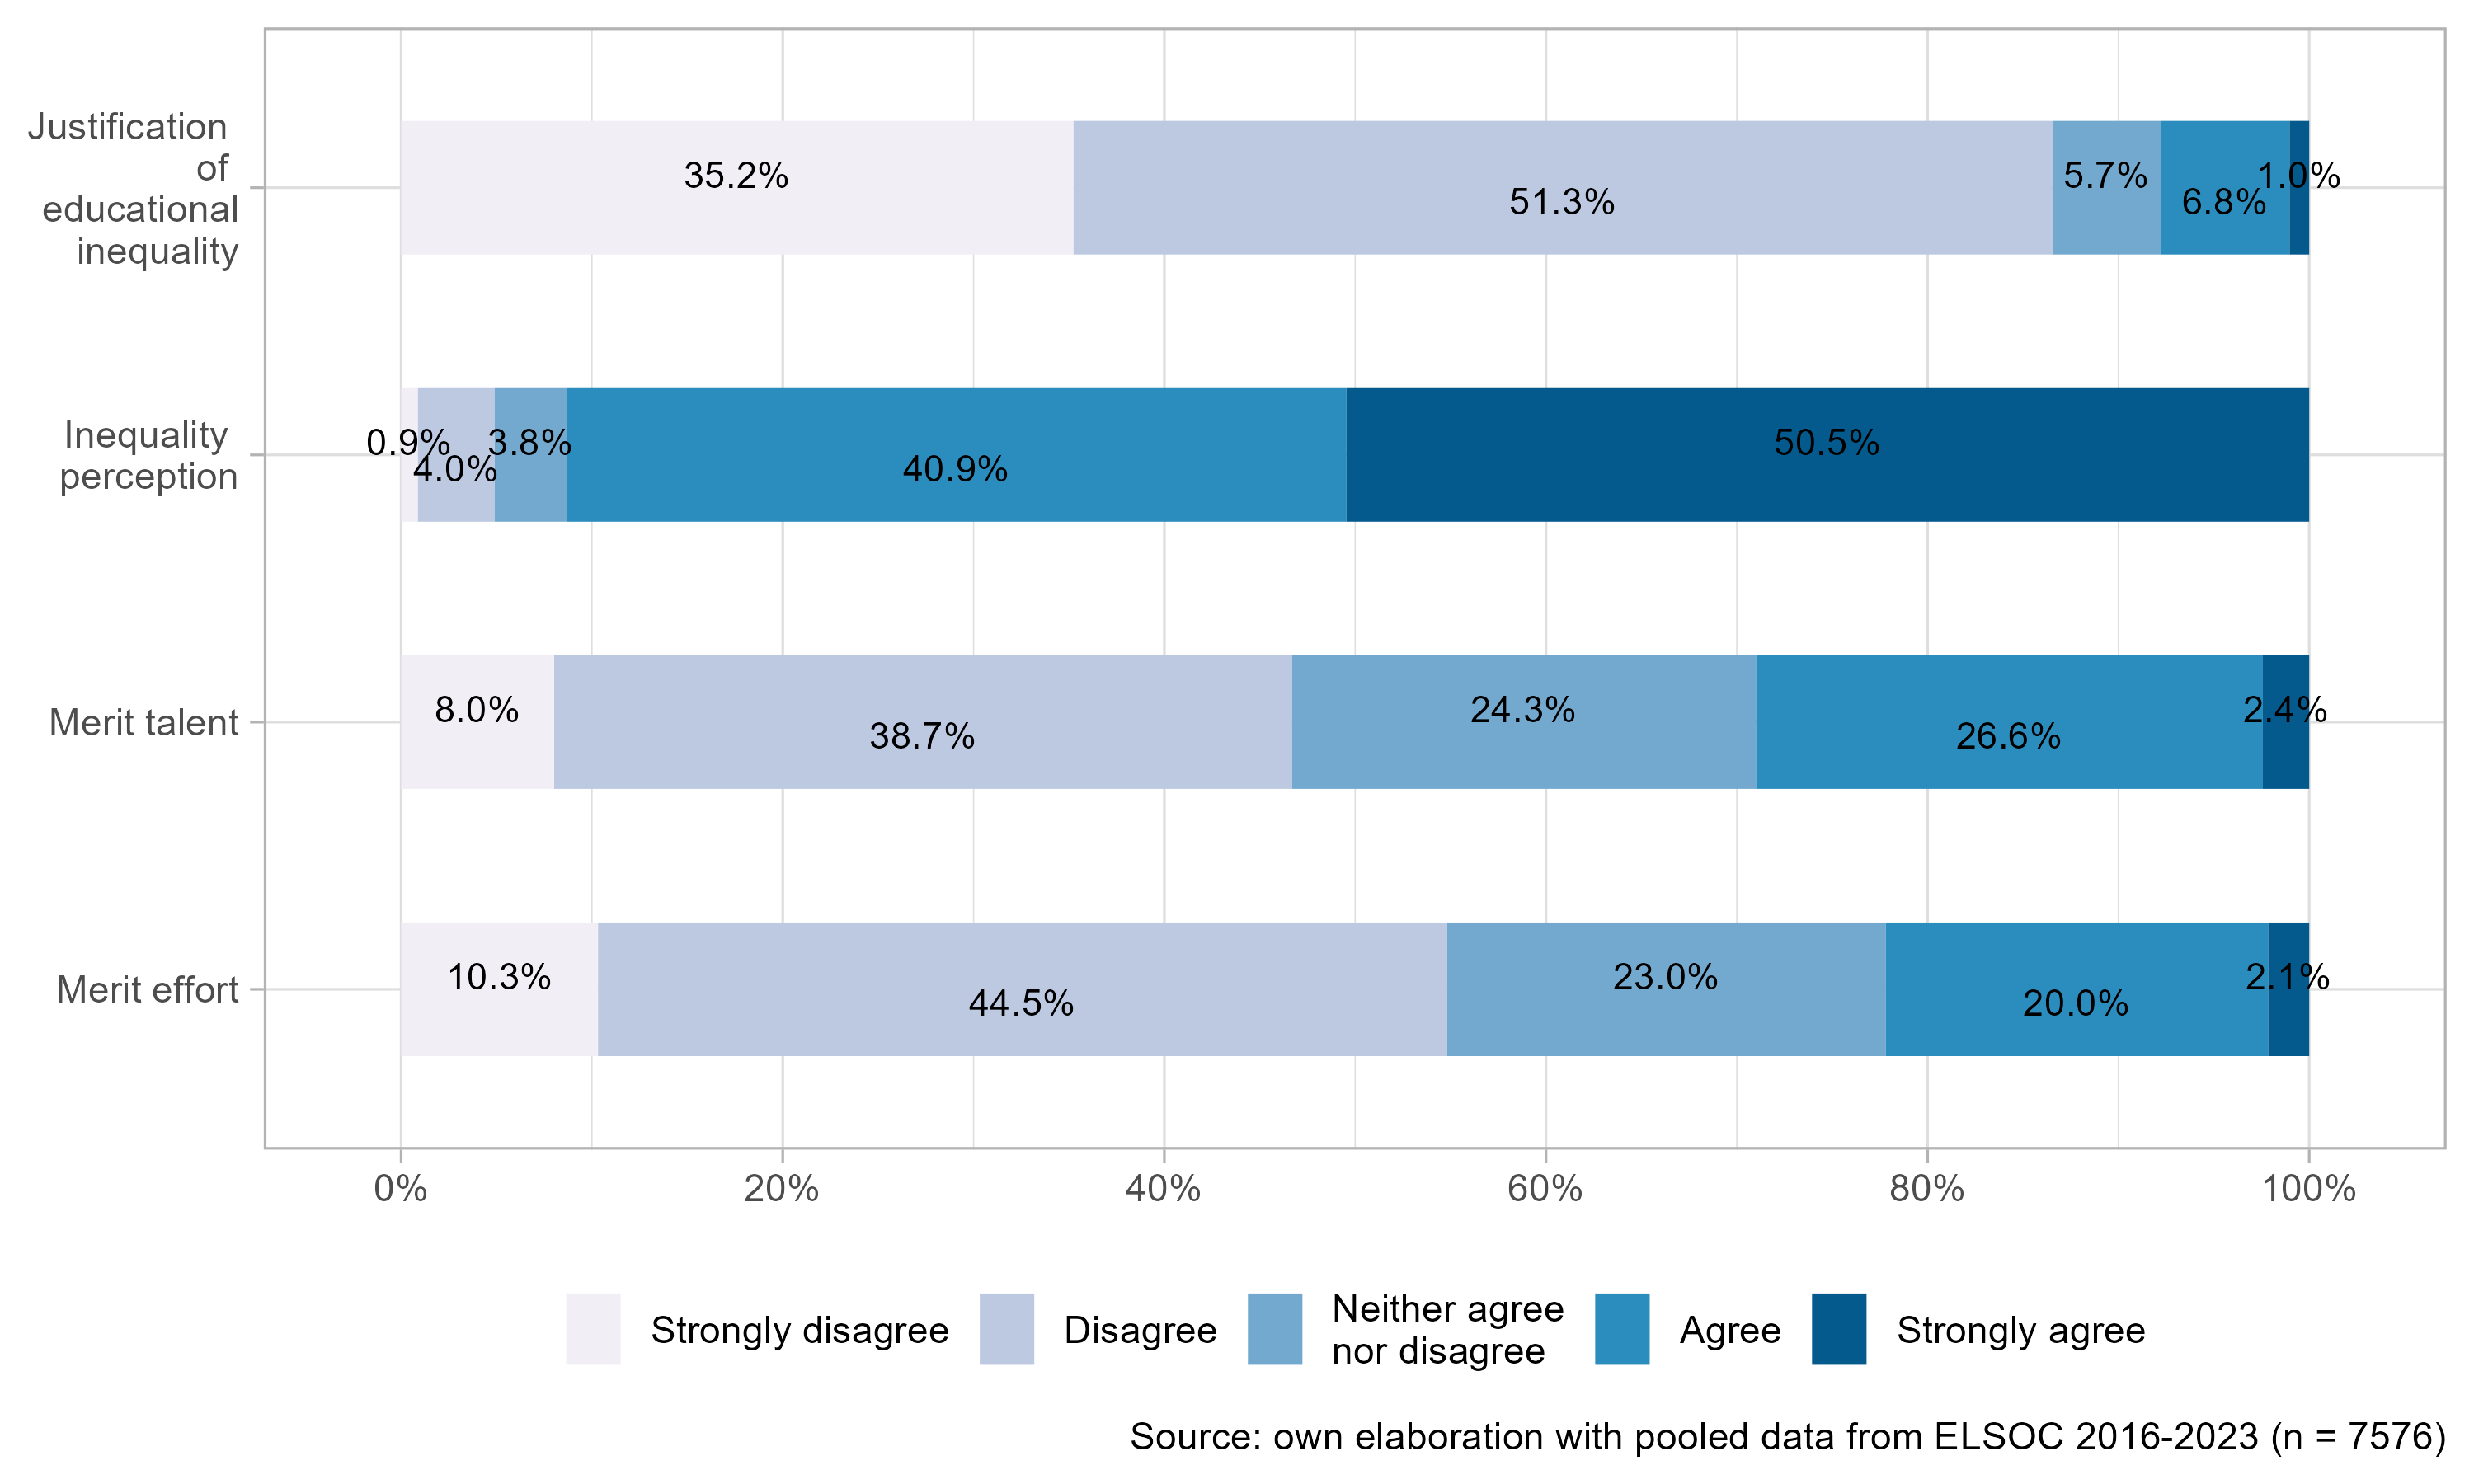
\includegraphics[width=0.85\textwidth,height=\textheight]{output/graphs/merit_plot.png}

}

\caption{\label{fig-frecuencies}Frequency of responses for justification
of educational inequality, perception of inequality, and perception of
meritocracy for all the years analyzed}

\end{figure}%

For testing the hypothesis regarding status we included educational
level and household income quintiles, as well as subjective social
status. Finally, political identification on a left-right scale, age,
and gender were included as control variables.
Table~\ref{tbl-descriptives} shows the whole set of independent
variables, the corresponding items, response categories, and
frequencies.

\begin{longtable}[]{@{}l@{}}
\caption{Independent variables}\label{tbl-descriptives}\tabularnewline
\toprule\noalign{}
\endfirsthead
\endhead
\bottomrule\noalign{}
\endlastfoot
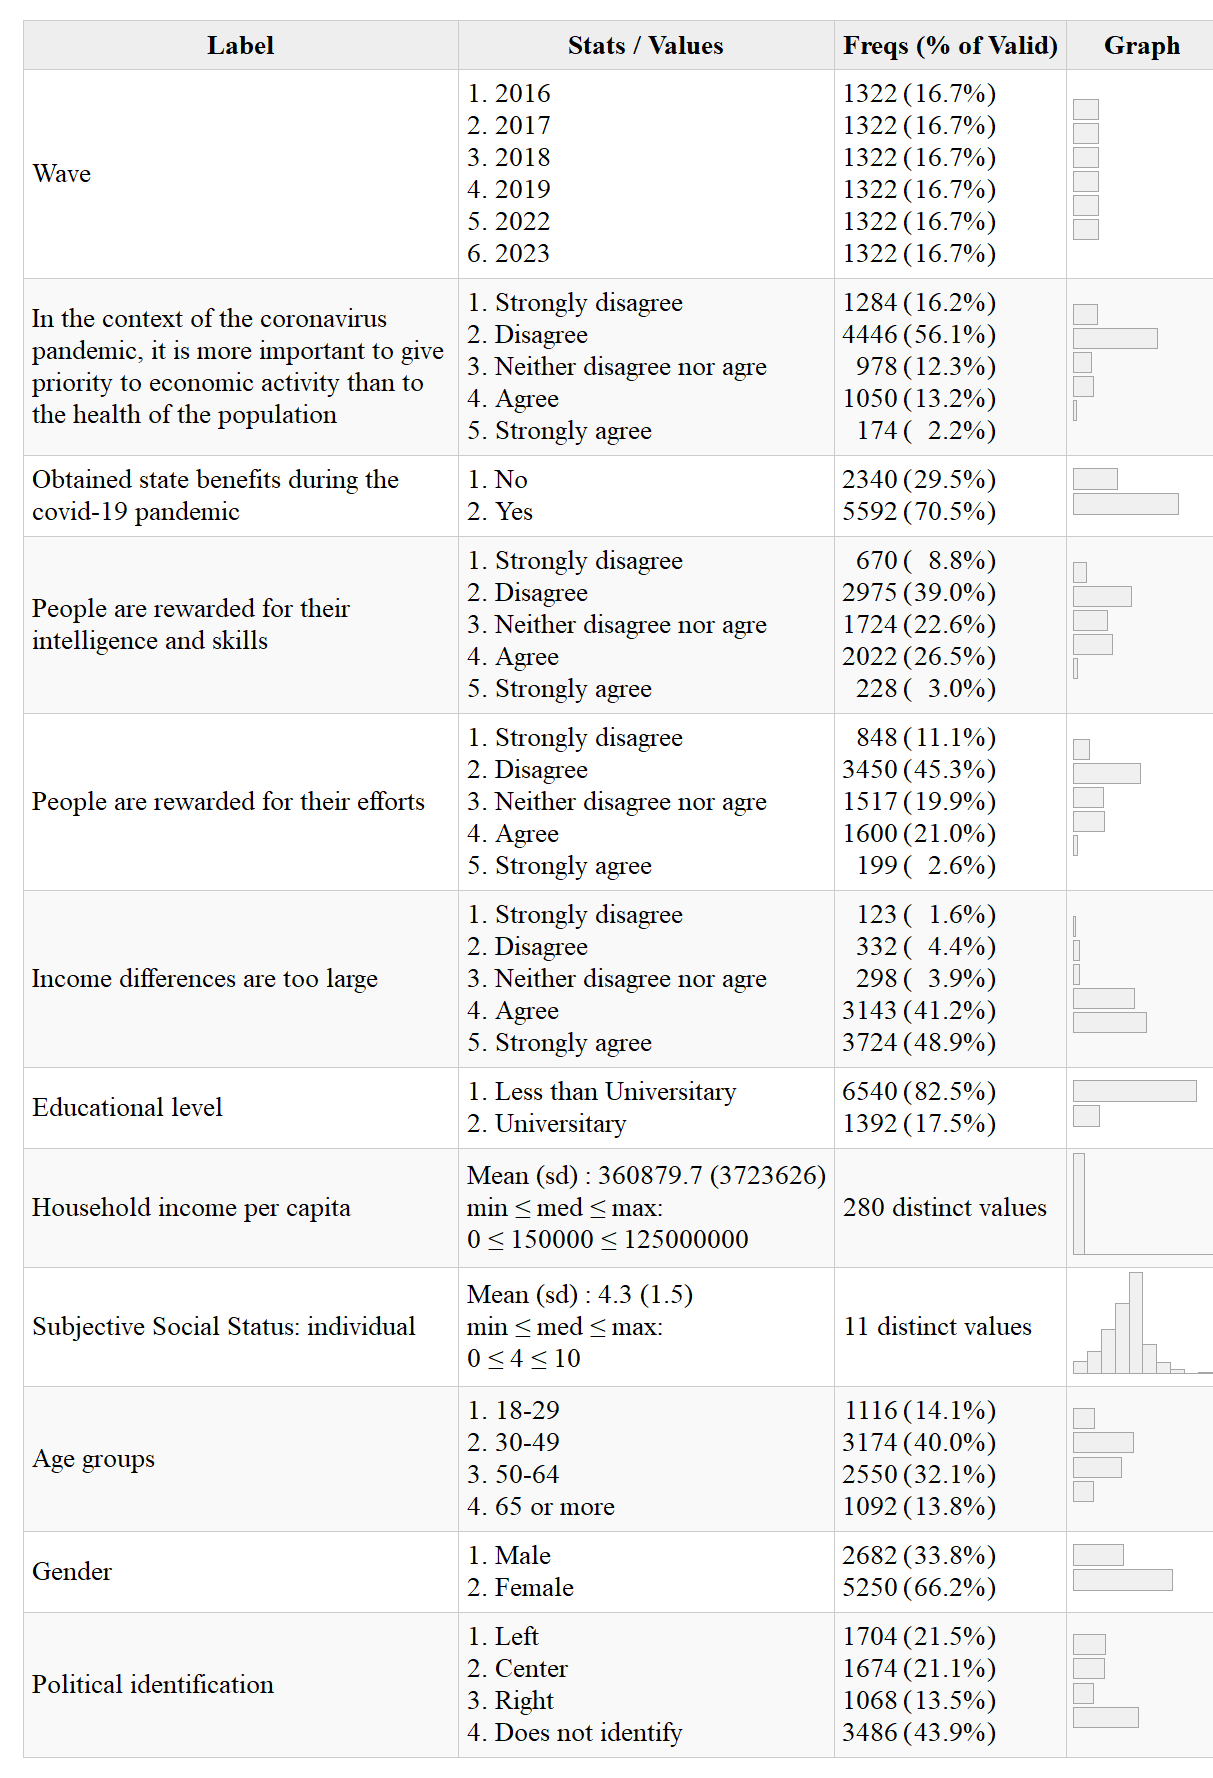
\includegraphics{output/tables/desc02.png} \\
\end{longtable}

\subsection{Methods}\label{methods}

Given the hierarchical structure of the data (observations nested in
survey waves), we estimated a series of longitudinal multilevel models
(Singer and Willett 2009). Such an approach is suited to account for the
shared variance among units (in this case individuals), adjusting the
estimation of the standard errors. The linear multilevel models are
estimated using the R library ``lme4'' (Singer and Willett 2009, 4).

\section{Results}\label{results}

\begin{figure}[H]

\centering{

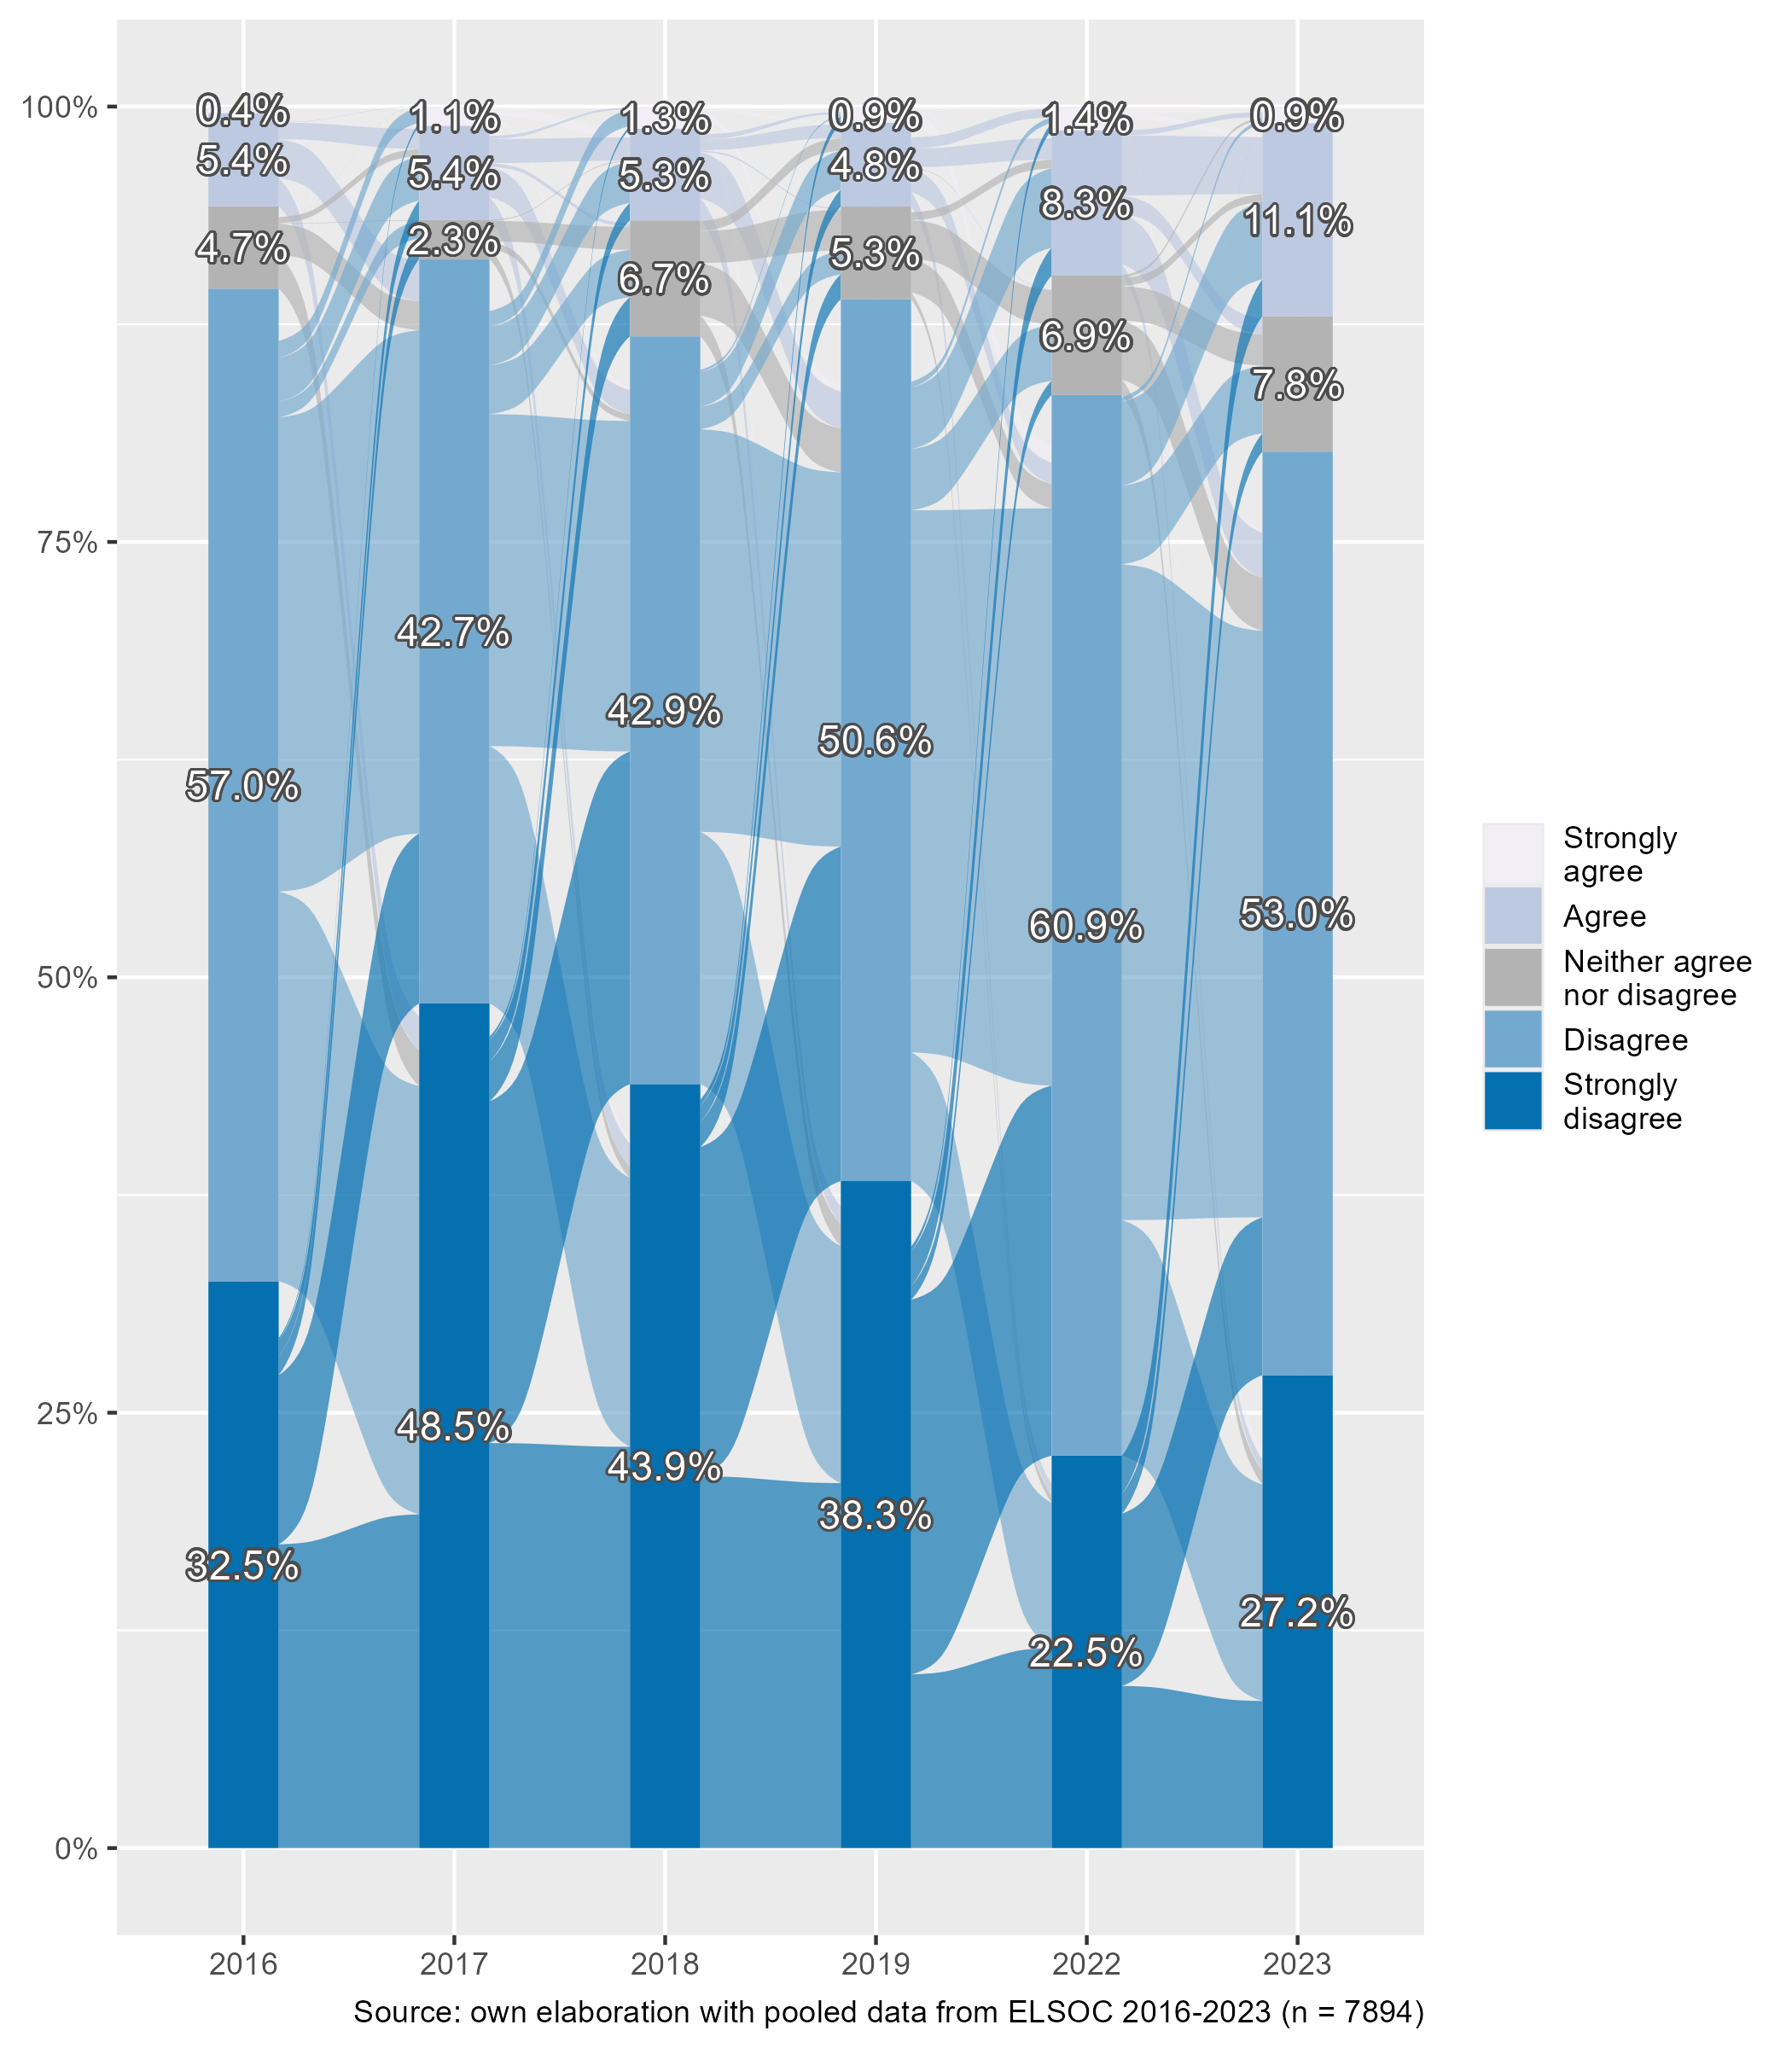
\includegraphics[width=0.85\textwidth,height=\textheight]{output/graphs/alluvial_dep.png}

}

\caption{\label{fig-alluvial}Change in the justification of educational
inequality over time (2016-2022)}

\end{figure}%

Figure~\ref{fig-alluvial} illustrates yearly frequencies in the
justification of educational inequality between 2016 and 2022. Each year
represents stacked percentual frequencies, and the flows in between
reflect the within-subject change of opinions from one year to the next,
as we are using longitudinal panel data (Rosvall and Bergstrom 2010).
For instance, of the 32.2\% who strongly disagreed with inequality
justification in 2016, about half of them kept responding the same in
2017, whereas the other half shifted their opinion to other response
categories. In general, the large majority - between 80 and 90\% -
disagrees with the justification of educational inequality throughout
the years. Despite this overall tendency, we also observe that the
disagreement with inequality justification (disagree + strongly
disagree) tends to go down in the last wave. This change is mostly a
result of the radical decrease in the lowest response category (strongly
disagree), which diminishes to half when compared with previous years.

\begin{figure}[H]

\centering{

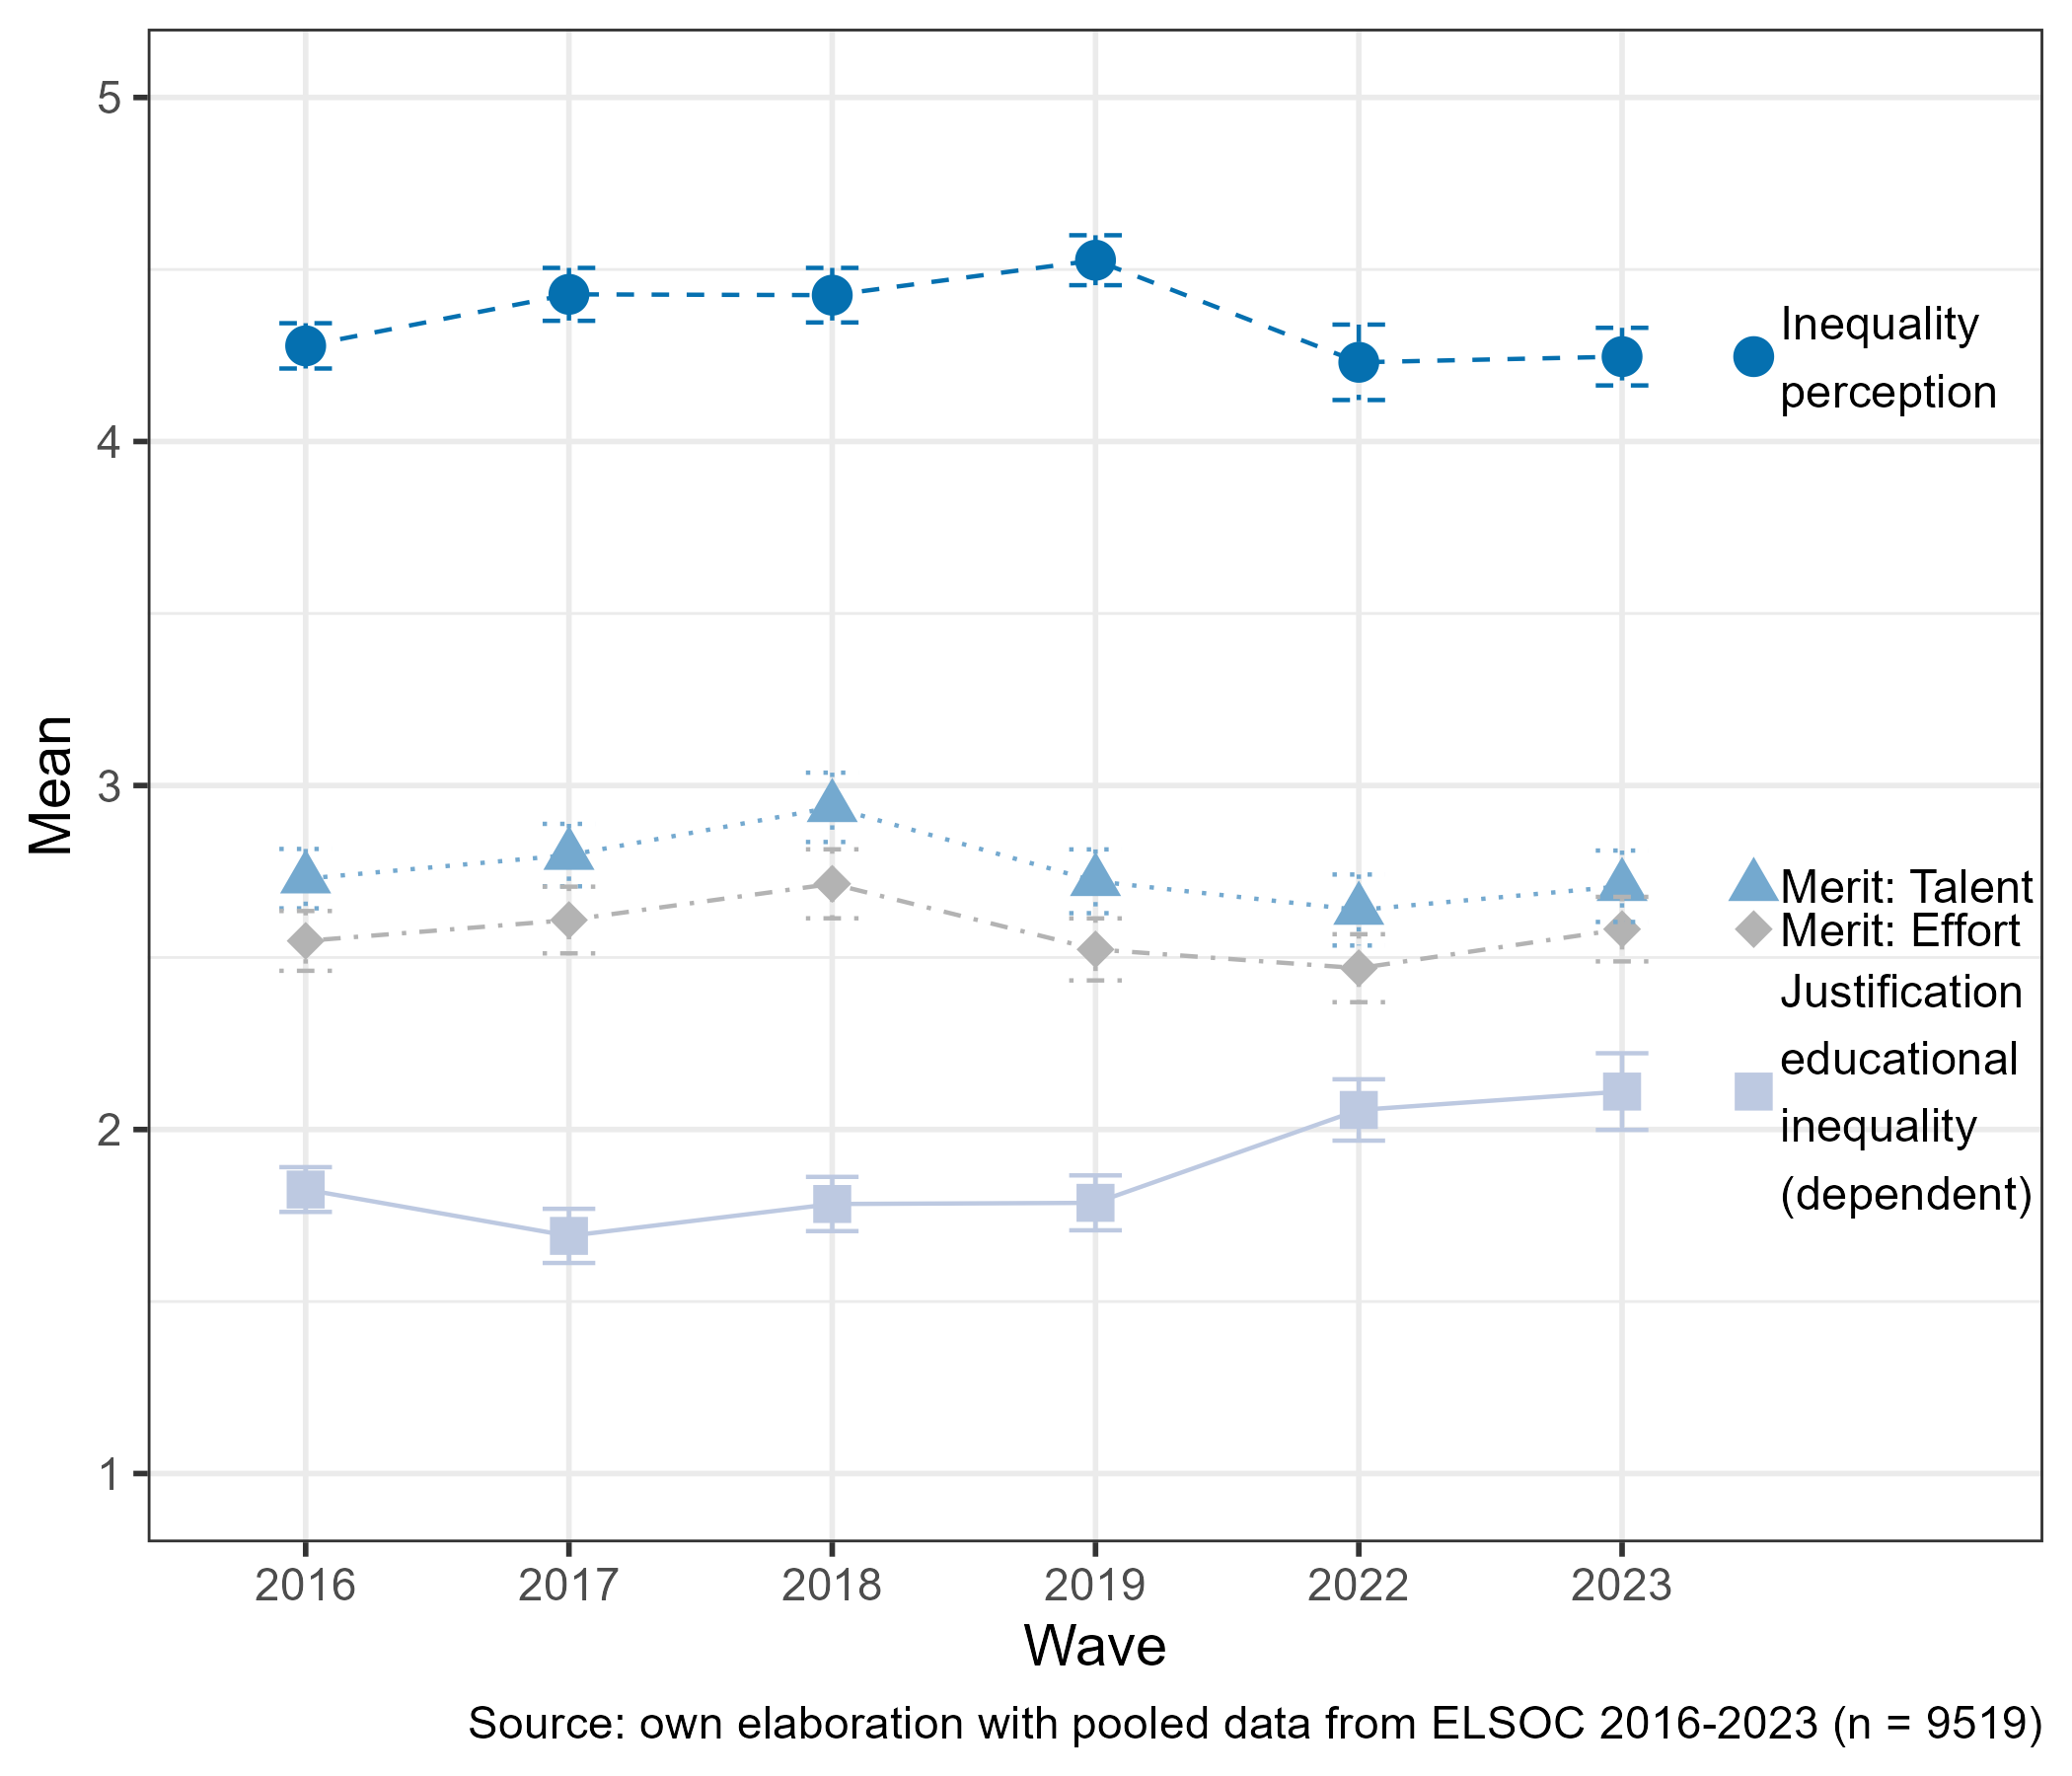
\includegraphics[width=0.85\textwidth,height=\textheight]{output/graphs/years_plot.png}

}

\caption{\label{fig-means}Change in the mean of justification of
educational inequality, perception of inequality, and perception of
meritocracy over the years}

\end{figure}%

Figure~\ref{fig-means} shows the average changes in the main variables
considered for this study. Here we observe that the justification of
educational inequality has the lowest average throughout the years when
compared with the other (independent) variables, whereas the highest
average is consistently represented by inequality perception.
Interestingly, in the last wave of the study (2022) the justification of
inequality increases whereas the perception of inequality decreases. As
the merit variables are concerned, they show a very similar pattern in
terms of averages and changes over the years, being the perception of
meritocracy related to effort always lower than the one associated with
talent.

\begin{figure}[H]

\centering{

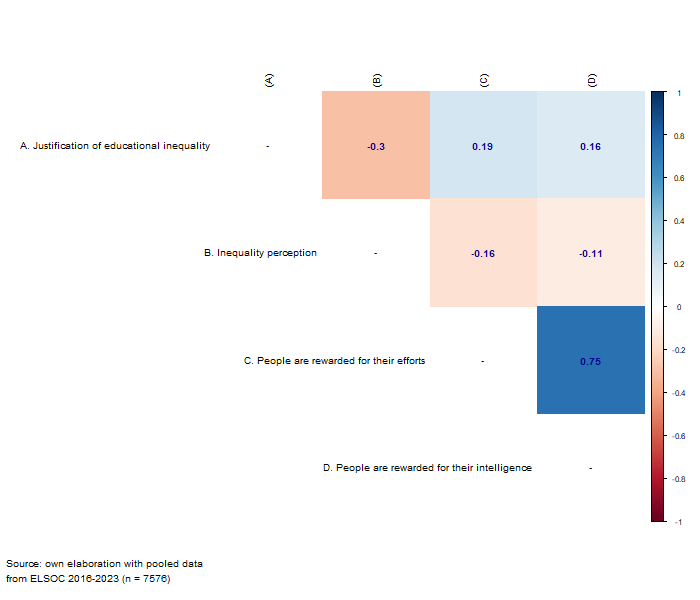
\includegraphics[width=0.85\textwidth,height=\textheight]{output/graphs/corr.png}

}

\caption{\label{fig-correlation}Correlation matrix of justification of
educational inequality, perception of inequality, and perception of
meritocracy for all the years analyzed}

\end{figure}%

Figure~\ref{fig-correlation} presents a correlation matrix of the main
variables analyzed, using data from all survey waves. In this matrix,
the correlations vary between low and moderate values. Justification of
economic inequality depicts a moderate and negative association with the
perception of inequality (\emph{r}=-0.29, p\textless.01) and a moderate
and positive association with both meritocracy perception variables
(\emph{r}=0.18, p\textless.01; \emph{r}=0.15, p\textless.01). Regarding
the perception of inequality, it presents a moderate and negative
association with both meritocracy perception variables (\emph{r}=-0.15,
p\textless.01; \emph{r}=-0.10, p\textless.01). Finally, the two
meritocracy variables present a high and positive association with each
other (\emph{r}=0.74, p\textless.01).

\subsection{Multivariate analysis}\label{multivariate-analysis}

Table~\ref{tbl-multilevel} shows the multilevel estimation results for
the justification of educational inequality. Model 1 includes the survey
waves to estimate intertemporal changes in the dependent variable.
Taking 2016 as a reference point, we can observe a staggered decrease in
2017 (\(\beta\)=-0.15, p\textless.001), 2018 (\(\beta\)=-0.06,
p\textless.05), and 2019 (\(\beta\)=-0.07, p\textless.01). Nevertheless,
in the last wave of 2022 there is a radical increase in level of
justification of economic inequality (\(\beta\)=0.21, p\textless.001),
suggesting a non-linear change in this variable. Attempting to model
this path of change over time, Model 2 incorporates time (survey waves)
as a continuous variable as well as its quadratic term, representing the
nonlinear association initially observed in Model 1. On the one hand,
the survey wave depicts a negative association, expressing an average
decrease in inequality justification over time, but on the other hand,
the quadratic wave term is positive, indicating the reversion of this
path in the last measurement point.

Model 3 adds the sociodemographic variables, where having a higher
income and being older (65 or older compared to 18-29) have a
significant and positive influence on the justification of educational
inequality. On the contrary, the gender variable has a negative effect,
expressing that women on average justify less inequality in education
when compared to males. Educational level and subjective social status
are not shown in this table for the sake of space (as they do not
exhibit significant effects), but the complete estimation of the models
is presented in the appendix. Model 3 also includes the control
variables, where identifying oneself with the center, right-wing, or
when reporting no political identification, has a significant and
positive association on the justification of educational inequality -
when compared to being left-wing oriented. Inequality perception is
added in Model 4, showing a negative association with the justification
of educational inequality as hypothesized, remaining stable when
controlling for the rest of the variables.

Models 5 and 6 introduce the meritocratic variables: talent (if
intelligence and abilities are rewarded in society) and effort (if
efforts are rewarded in society). In line with our hypotheses, the
perception that talent is rewarded has a positive influence on the
justification of educational inequality in Model 5 (\(\beta\)=0.04,
p\textless.01). However, when controlling for the perception that effort
is rewarded, this effect is no longer significant. In this sense, Model
6 shows that the perception that effort is rewarded in society is not
only positively associated with the justification of educational
inequality (\(\beta\)=0.05, p\textless.01), but it has a larger weight
than the perception of talent.

\begin{table}

\caption{\label{tbl-multilevel}Multilevel longitudinal models for the
justification of inequality in education}

\centering{

Statistical models

~

Model 1

Model 2

Model 3

Model 4

Model 5

Model 6

Intercept

1.84***

1.87***

1.80***

2.39***

2.22***

2.13***

~

(0.02)

(0.03)

(0.09)

(0.10)

(0.10)

(0.10)

Wave (Ref.= Wave 2016)

~

~

~

~

~

~

~

~

~

~

~

~

~

~~~~~Wave 2017

-0.14***

~

~

~

~

~

~

(0.03)

~

~

~

~

~

~~~~~Wave 2018

-0.04

~

~

~

~

~

~

(0.03)

~

~

~

~

~

~~~~~Wave 2019

-0.04

~

~

~

~

~

~

(0.03)

~

~

~

~

~

~~~~~Wave 2022

0.23***

~

~

~

~

~

~

(0.03)

~

~

~

~

~

~~~~~Wave 2023

0.28***

~

~

~

~

~

~

(0.03)

~

~

~

~

~

Wave

~

-0.08***

-0.08***

-0.05**

-0.06**

-0.06**

~

~

(0.02)

(0.02)

(0.02)

(0.02)

(0.02)

Wave\^{}2

~

0.02***

0.02***

0.01***

0.01***

0.01***

~

~

(0.00)

(0.00)

(0.00)

(0.00)

(0.00)

Household Income (Ref.= Quintile 1)

~

~

~

~

~

~

~

~

~

~

~

~

~

~~~~~Quintile 2

~

~

0.05

0.04

0.04

0.04

~

~

~

(0.05)

(0.05)

(0.05)

(0.05)

~~~~~Quintile 3

~

~

0.10

0.09

0.09

0.10

~

~

~

(0.05)

(0.05)

(0.05)

(0.05)

~~~~~Quintile 4

~

~

0.11

0.11*

0.11*

0.11*

~

~

~

(0.06)

(0.05)

(0.05)

(0.05)

~~~~~Quintile 5

~

~

0.15**

0.15**

0.16**

0.16**

~

~

~

(0.06)

(0.06)

(0.06)

(0.06)

~~~~~Quintile (No information)

~

~

0.16*

0.17*

0.18*

0.17*

~

~

~

(0.08)

(0.08)

(0.08)

(0.08)

Age (Ref.= 18-29)

~

~

~

~

~

~

~

~

~

~

~

~

~

~~~~~Age 30-49

~

~

-0.02

-0.01

-0.01

-0.02

~

~

~

(0.05)

(0.05)

(0.05)

(0.05)

~~~~~Age 50-64

~

~

0.03

0.04

0.03

0.03

~

~

~

(0.05)

(0.05)

(0.05)

(0.05)

~~~~~Age 65 or more

~

~

0.14*

0.14*

0.13*

0.12*

~

~

~

(0.06)

(0.06)

(0.06)

(0.06)

Gender (Ref. Male)

~

~

-0.10**

-0.10**

-0.09**

-0.08*

~

~

~

(0.03)

(0.03)

(0.03)

(0.03)

Pol. pos (Ref.= Left)

~

~

~

~

~

~

~

~

~

~

~

~

~

~~~~~Center

~

~

0.08

0.07

0.07

0.07

~

~

~

(0.05)

(0.05)

(0.05)

(0.05)

~~~~~Right

~

~

0.28***

0.26***

0.25***

0.25***

~

~

~

(0.05)

(0.05)

(0.05)

(0.05)

~~~~~Does not identify

~

~

0.09*

0.08

0.08

0.08

~

~

~

(0.04)

(0.04)

(0.04)

(0.04)

Inequality perception

~

~

~

-0.15***

-0.14***

-0.14***

~

~

~

~

(0.01)

(0.01)

(0.01)

Merit: Talent

~

~

~

~

0.06***

0.01

~

~

~

~

~

(0.01)

(0.01)

Merit: Effort

~

~

~

~

~

0.08***

~

~

~

~

~

~

(0.01)

BIC

37741.49

37740.80

37897.19

37723.09

37697.94

37668.38

Num. obs.

9519

9519

9519

9519

9519

9519

Num. groups: Individuals

1701

1701

1701

1701

1701

1701

Var: Individuals (Intercept)

0.18

0.18

0.17

0.17

0.16

0.16

Var: Residual

0.53

0.53

0.53

0.52

0.52

0.52

*** p \textless{} 0.001; ** p \textless{} 0.01; * p \textless{} 0.05.
Note: Model 3 to 6 are controlled by educational level, and subjective
social status with no significant effects.

}

\end{table}%

\begin{table}

\caption{\label{tbl-interact}}

\centering{

Statistical models

~

Model 1

Model 2

Model 3

Intercept

2.13***

1.96***

2.10***

~

(0.10)

(0.11)

(0.11)

Wave

-0.06**

-0.03

-0.06**

~

(0.02)

(0.02)

(0.02)

Wave\^{}2

0.01***

0.01***

0.01***

~

(0.00)

(0.00)

(0.00)

Merit: Talent

0.01

0.04

0.01

~

(0.01)

(0.02)

(0.01)

Merit: Effort

0.08***

0.08***

0.07**

~

(0.01)

(0.01)

(0.02)

Wave * Merit: Talent

~

-0.01

~

~

~

(0.00)

~

Wave * Merit: Effort

~

~

0.00

~

~

~

(0.00)

BIC

37668.38

36196.86

36307.66

Num. obs.

9519

9519

9519

Num. groups: Individuals

1701

1701

1701

Var: Individuals (Intercept)

0.16

0.96

0.88

Var: Residual

0.52

0.36

0.37

Var: Individuals Wave

~

0.02

0.02

Var: Individuals Merit: Talent

~

0.10

~

Cov: Individuals (Intercept) Wave

~

-0.05

-0.05

Cov: Individuals (Intercept) Merit: Talent

~

-0.26

~

Cov: Individuals Wave Merit: Talent

~

-0.00

~

Var: Individuals Merit: Effort

~

~

0.10

Cov: Individuals (Intercept) Merit: Effort

~

~

-0.24

Cov: Individuals Wave Merit: Effort

~

~

0.00

\item *

** p \textless{} 0.001; ** p \textless{} 0.01; * p \textless{} 0.05.
Note: All the models are controlled by educational level, income
quintile, subjective social status, age, gender, political position, and
inequality perception

}

\end{table}%

In this final part of the analysis, we contrast longitudinal hypotheses
regarding changes in the relationship between meritocracy and
justification of economic inequality over time. In hypothesis 5 we
proposed that the association between the perception of meritocracy and
inequality justification mitigates over time, as meritocratic ideals
could have weakened due to critical situations associated with the COVID
pandemic. We test this hypothesis through interaction effects, displayed
in Table~\ref{tbl-interact}. Model 1 is shown as a baseline model, it is
the same as Model 6 in Table~\ref{tbl-interact} but it only displays the
variables involved in the interaction for the sake of space (all other
variables are controlled for). Model 2 adds the interaction between the
perception of meritocracy based on talent and time (panel wave), whereas
Model 3 does the same but now for the perception of meritocracy related
to effort. As observed, only the effort variable shows a significant
interaction with the time variable (\(\beta\)=0.01, p\textless.05),
meaning that, on average, the association between the perception of
meritocracy based on effort and the justification of inequality
increases by 0.01 points in every measurement point.

\section{Discussion and conclusions}\label{discussion-and-conclusions}

Our research sought to examine the relationship between the perception
of meritocracy and the justification of inequality in education from a
longitudinal perspective amid the health crisis generated by the
COVID-19 pandemic. In general, our results showed mixed evidence about
our hypotheses. Whereas we find support for the association between the
perception of meritocracy and justification of inequality across time,
the analyses that involved changes in justification of inequality are
against our initial proposal. We argued that in times of crisis, greater
exposure to risk due to the health context would result in a lower
justification of inequality by citizens. In this regard, longitudinal
models showed that the justification of inequality in education is far
from being linear, and whereas a decreasing pattern was found between
2017 and 2019, there is a striking increase in the last measurement
point (2022), after the peak of the COVID pandemic. As we mentioned at
the beginning, given our data limitations it is not possible to
attribute such changes only to the pandemic and the related economic and
social crises. As in the Chilean case, the pandemic period occurred
along with a constitutional process, disentangling different forces
driving public opinion it becomes difficult and deserves further
qualitative and quantitative studies. A closer look to the political
environment during the last year in the country could give additional
hints. Some recent studies have argued that the election of a far
left-wing constitutional assembly during this period generated a
backslash effect, mainly due to several scandals that led to the
delegitimation of this assembly. This could have driven preferences in a
conservative direction, which was reflected in the election of a
right-wing second assembly after the failed first constitutional process
(Palanza and Sotomayor 2023; Sazo 2023).

Regarding the status position, our central hypothesis was that
individuals in more advantaged situations and with greater resources
would tend to defend their interests and justify greater education
inequality (\(H_2\)). In this regard, our results show a positive and
robust relationship between income and the justification of inequality,
which would align with our original hypothesis based on the rational
interests of the better-off that would lead to a larger inequality
justification. Besides status, we also considered inequality perception,
as the literature on attitudes toward inequality has argued that a
greater justification of inequality is associated with its perceived
magnitude (\(H_3\)). Consistent with this hypothesis, our results showed
that, throughout the years, a larger perceived economic inequality
motivates a lower justification of inequality in education.

The main focus of this study was on the relationship between meritocracy
and justification of inequality, arguing that those who perceive that
the society in which they live complies with meritocratic principles,
would be more inclined to justify inequality in education (\(H_4\)). At
first look, the results are consistent with the hypothesis; however,
some nuances are worth attending concerning different aspects of
meritocracy, namely effort and talent. Our results are favorable for the
effort dimension but not confirmed for the talent dimension. In other
words, the perception of meritocracy in terms of rewarded effort is more
relevant in justifying access to education than the perception of
talent. This could be explained as that talent could be more associated
with luck in terms of random assignment, and in this terms would not be
enough reason (as it is effort) to justify educational inequality.

Finally, as our first hypothesis supported, we expected that the
relationship between meritocratic perceptions and justification would
tend to diminish over time. However, longitudinal evidence shows that
the perception of meritocracy linked to effort strengthens its relation
with the justification of inequality in education, against the temporal
change hypothesis (\(H_5\)). In other words, meritocracy seems to gain
force concerning justifying inequality and not the other way around as
we expected given the social context in the post-covid era. An
alternative interpretation is that in times of high exposure to risk,
people tend to stick more to narratives that provide greater security
regardless of the rest of the society - such as individual effort -,
which might also be accompanied by lower degrees of solidarity to
safeguard the well-being of themselves and their surrounding close
peers. Again, this certainly needs further studies that include
additional specific conceptual and methodological approaches to this
phenomenon.

Among the limitations of our study, we can mention at least three.
First, we know that inequalities in education can manifest themselves in
terms of outcomes as well as in areas such as access to social services
in education as part of welfare policies. In this regard, the construct
that we have captured with our indicator can be framed more in the
latter, while the evaluation of justice involved in this process does
not consider aspects such as equality of educational opportunities or
observable outcomes such as the performance of individual or educational
institutions. Second, as it has been established by recent research
(Castillo et al. 2023), the perception of meritocracy can be understood
through individual attributions regarding effort and talent, but also as
a function of structural aspects such as family of origin status or
social capital. In this sense, the available measurements restricted us
to the use of single indicators for effort and talent, and further
research should consider improving the measurement quality in this
regard. Finally, there are limitations involving the longitudinal
dimension of the data used. Given constraints for data collection during
the pandemic, the ELSOC study had to shorten the questionnaire in 2021
and unfortunately, the educational justice indicator was excluded from
that survey. Consequently, the results of temporal change have to be
considered carefully, and further data waves could give us more
information on this matter.

The capabilities of the ELSOC longitudinal database are not limited to
micro-level estimates. In this regard, thanks to the sampling strategy
of the survey, it would be possible to make contextual estimates at the
municipality level in future studies. For instance, statistical models
could include contextual information from administrative data sources,
allowing testing for hypotheses that include contextual socioeconomic
inequality as well as its dynamics over time. Furthermore, this dataset
could be used for comparing inequality justification in policy areas
besides education, such as health and pensions. Future studies may shed
light on how meritocratic perceptions and beliefs affect differently
such areas and their changes over time, which would give relevant hints
from social sciences for the discussion about societal and cultural
changes as well as their impacts on solidarity and social cohesion.

\section{References}\label{references}

\phantomsection\label{refs}
\begin{CSLReferences}{1}{0}
\bibitem[\citeproctext]{ref-barry_theories_1989}
Barry, Brian. 1989. \emph{Theories of Justice}. A Treatise on Social
Justice 1. Berkeley: Univ. of California Pr.

\bibitem[\citeproctext]{ref-batruch_belief_2023}
Batruch, Anatolia, Jolanda Jetten, Herman Van De Werfhorst, Céline
Darnon, and Fabrizio Butera. 2023. {``Belief in {School Meritocracy} and
the {Legitimization} of {Social} and {Income Inequality}.''}
\emph{Social Psychological and Personality Science} 14 (5): 621--35.
\url{https://doi.org/10.1177/19485506221111017}.

\bibitem[\citeproctext]{ref-bell_politics_2020}
Bell, Elizabeth. 2020. {``The {Politics} of {Designing Tuition-Free
College}: {How Socially Constructed Target Populations Influence Policy
Support}.''} \emph{The Journal of Higher Education} 91 (6): 888--926.
\url{https://doi.org/10.1080/00221546.2019.1706015}.

\bibitem[\citeproctext]{ref-bellei_estudio_2013}
Bellei, Cristián. 2013. {``El Estudio de La Segregaci{ó}n
Socioecon{ó}mica y Acad{é}mica de La Educaci{ó}n Chilena.''}
\emph{Estudios Pedag{ó}gicos (Valdivia)} 39 (1): 325--45.
\url{https://doi.org/10.4067/S0718-07052013000100019}.

\bibitem[\citeproctext]{ref-breznau_welfare_2021}
Breznau, Nate. 2021. {``The Welfare State and Risk Perceptions: The
{Novel Coronavirus Pandemic} and Public Concern in 70 Countries.''}
\emph{European Societies} 23 (sup1): S33--46.
\url{https://doi.org/10.1080/14616696.2020.1793215}.

\bibitem[\citeproctext]{ref-busemeyer_welfare_2020}
Busemeyer, Marius R., and Torben Iversen. 2020. {``The {Welfare State}
with {Private Alternatives}: {The Transformation} of {Popular Support}
for {Social Insurance}.''} \emph{The Journal of Politics} 82 (2):
671--86. \url{https://doi.org/10.1086/706980}.

\bibitem[\citeproctext]{ref-Castillo2011}
Castillo, Juan Carlos. 2011. {``Legitimacy of {Inequality} in a {Highly
Unequal Context}: {Evidence} from the {Chilean Case}.''} \emph{Social
Justice Research} 24 (4): 314--40.
\url{https://doi.org/10.1007/s11211-011-0144-5}.

\bibitem[\citeproctext]{ref-Castillo2012a_justice}
---------. 2012. {``Is {Inequality Becoming Just}? {Changes} in {Public
Opinion} about {Economic Distribution} in {Chile}.''} \emph{Bulletin of
Latin American Research} 31 (1): 1--18.
\url{https://doi.org/10.1111/j.1470-9856.2011.00605.x}.

\bibitem[\citeproctext]{ref-castillo_perception_2022}
Castillo, Juan Carlos, Juan-Diego García-Castro, and Martín Venegas.
2022. {``Perception of Economic Inequality: Concepts, Associated Factors
and Prospects of a Burgeoning Research Agenda.''} \emph{International
Journal of Social Psychology} 37 (1): 180--207.
\url{https://doi.org/10.1080/02134748.2021.2009275}.

\bibitem[\citeproctext]{ref-castillo_multidimensional_2023}
Castillo, Juan Carlos, Julio Iturra, Luis Maldonado, Jorge Atria, and
Francisco Meneses. 2023. {``A {Multidimensional Approach} for {Measuring
Meritocratic Beliefs}: {Advantages}, {Limitations} and {Alternatives} to
the {ISSP Social Inequality Survey}.''} \emph{International Journal of
Sociology}, October, 1--25.
\url{https://doi.org/10.1080/00207659.2023.2274712}.

\bibitem[\citeproctext]{ref-confortiLegitimationInequalityAmerican1992}
Conforti, Joseph M. 1992. {``The Legitimation of Inequality in
{American} Education.''} \emph{The Urban Review} 24 (4): 227--38.
\url{https://doi.org/10.1007/BF01108357}.

\bibitem[\citeproctext]{ref-corvalanMercadoEscolarLibertad2016}
Corvalán, Javier, Alejandro Carrasco, and J. E. García-Huidobro, eds.
2016. \emph{Mercado Escolar: {Libertad}, Diversidad y Desigualdad}. 1st
ed. Santiago: Ediciones UC. \url{https://doi.org/10.2307/j.ctv14rmrhn}.

\bibitem[\citeproctext]{ref-darmodyImpactsCOVID19Control2021}
Darmody, Merike, Emer Smyth, and Helen Russell. 2021. {``Impacts of the
{COVID-19 Control Measures} on {Widening Educational Inequalities}.''}
\emph{YOUNG} 29 (4): 366--80.
\url{https://doi.org/10.1177/11033088211027412}.

\bibitem[\citeproctext]{ref-dayPerceivedIdealInequality2023}
Day, Martin V., and Michael I. Norton. 2023. {``Perceived and {Ideal
Inequality} in {University Endowments} in the {United States}.''}
\emph{Personality and Social Psychology Bulletin} 49 (8): 1151--65.
\url{https://doi.org/10.1177/01461672221083766}.

\bibitem[\citeproctext]{ref-elsoc_estudio_2022}
ELSOC, Survey Team. 2022. {``Estudio {Longitudinal Social} de
{Chile}.''} Harvard Dataverse. \url{https://doi.org/10.7910/dvn/0kirbj}.

\bibitem[\citeproctext]{ref-Evans2017}
Evans, M. D. R., and Jonathan Kelley. 2017. {``Communism, {Capitalism},
and {Images} of {Class}: {Effects} of {Reference Groups}, {Reality}, and
{Regime} in 43 {Nations} and 110,000 {Individuals}, 1987-2009.''}
\emph{Cross-Cultural Research} 51 (514): 315--59.
\url{https://doi.org/10.1177/1069397116677963}.

\bibitem[\citeproctext]{ref-Evans1992}
Evans, M. D. R., Jonathan Kelley, and Tamas Kolosi. 1992. {``Images of
{Class}: {Public Perceptions} in {Hungary} and {Australia}.''}
\emph{American Sociological Review} 57 (4): 461.
\url{https://doi.org/10.2307/2096095}.

\bibitem[\citeproctext]{ref-garcia-sanchez_creencias_2022}
García-Sánchez, Efraín, and Sofia De Carvalho. 2022. {``Las Creencias
Que Justifican La Desigualdad Moderan La Relaci{ó}n Entre El Estatus
Socioecon{ó}mico y El Apoyo a La Redistribuci{ó}n.''} \emph{Revista
Internacional de Sociolog{í}a} 80 (3): e210.
\url{https://doi.org/10.3989/ris.2022.80.3.21.29}.

\bibitem[\citeproctext]{ref-gimpelson_misperceiving_2018}
Gimpelson, Vladimir, and Daniel Treisman. 2018. {``Misperceiving
Inequality.''} \emph{Economics \& Politics} 30 (1): 27--54.
\url{https://doi.org/10.1111/ecpo.12103}.

\bibitem[\citeproctext]{ref-goldin_meritocracy_2000}
Goldin, Claudia. 2000. {``Meritocracy and {Economic Inequality}.
{Edited} by {Kenneth Arrow}, {Samuel Bowles}, and {Steven Durlauf} (
{Princeton}, {Princeton University Press}, 2000) 348 Pp.''}
\emph{Journal of Interdisciplinary History} 31 (3): 431a--433.
\url{https://doi.org/10.1162/jinh.2000.31.3.431a}.

\bibitem[\citeproctext]{ref-hadjar_meritokratie_2008}
Hadjar, Andreas. 2008. \emph{{Meritokratie als Legitimationsprinzip}}.
Wiesbaden: VS Verlag f{ü}r Sozialwissenschaften.

\bibitem[\citeproctext]{ref-hadler_why_2005}
Hadler, Markus. 2005. {``Why {Do People Accept Different Income
Ratios}?: {A Multi-level Comparison} of {Thirty Countries}.''}
\emph{Acta Sociologica} 48 (2): 131--54.
\url{https://doi.org/10.1177/0001699305053768}.

\bibitem[\citeproctext]{ref-hankivsky_introduction_2022}
Hankivsky, Olena, Marina Morrow, and Colleen Varcoe. 2022.
{``{INTRODUCTION Women}'s {Health} in {Canada}: {Critical Intersectional
Perspectives} on {Theory} and {Policy}.''} In \emph{Women's {Health} in
{Canada}}, edited by Marina Morrow, Olena Hankivsky, and Colleen Varcoe,
1--10. University of Toronto Press.
\url{https://doi.org/10.3138/9781442623958-003}.

\bibitem[\citeproctext]{ref-igliozziFairShareEffects2024}
Igliozzi, David, Yael Granot, and Victor Ottati. 2024. {``A Fair Share:
{Effects} of Disparity, Allocation Strategy and System Justification on
Perceptions of Policy Support in the Education Domain.''} \emph{European
Journal of Social Psychology}, February, ejsp.3040.
\url{https://doi.org/10.1002/ejsp.3040}.

\bibitem[\citeproctext]{ref-iturra_percepcion_2023}
Iturra, Julio, Juan Carlos Castillo, Catalina Rufs Orellana, and Luis
Maldonado. 2023. {``La Percepci{ó}n de Desigualdad Econ{ó}mica y Su
Influencia Sobre La Justificaci{ó}n de Las Diferencias de Ingreso
Leg{í}timas.''} \emph{Estudios Sociol{ó}gicos de El Colegio de M{é}xico}
41 (122): 309--52. \url{https://doi.org/10.24201/es.2023v41n122.2260}.

\bibitem[\citeproctext]{ref-janmaatSubjectiveInequalityReview2013}
Janmaat, Jan Germen. 2013. {``Subjective Inequality: {A} Review of
International Comparative Studies on People's Views about Inequality.''}
\emph{Archives Europeennes de Sociologie} 54 (3): 357--89.
\url{https://doi.org/10.1017/S0003975613000209}.

\bibitem[\citeproctext]{ref-jassoJusticeEarningsNew1978}
Jasso, Guillermina. 1978. {``On the {Justice} of {Earnings}: {A New
Specification} of the {Justice Evaluation Function}.''} \emph{American
Journal of Sociology} 83 (6): 1398--1419.
\url{https://www.jstor.org/stable/2778110}.

\bibitem[\citeproctext]{ref-joiko_cuasimercado_2019}
Joiko, Sara. 2019. {``{El cuasi-mercado educativo en Chile: desarrollo y
consecuencias}.''} \emph{Revista Electr{ó}nica Di{á}logos Educativos;
Vol. 12 N{ú}m. 23 (2012); 148-174}, April.

\bibitem[\citeproctext]{ref-jost_theory_2020}
Jost, John. 2020. \emph{A Theory of System Justification}. Cambridge,
Massachusetts: Harvard University Press.

\bibitem[\citeproctext]{ref-jost_psychology_2003}
Jost, John, and Orsolya Hunyady. 2003. {``The Psychology of System
Justification and the Palliative Function of Ideology.''} \emph{European
Review of Social Psychology} 13 (1): 111--53.
\url{https://doi.org/10.1080/10463280240000046}.

\bibitem[\citeproctext]{ref-kelleyLegitimationInequalityOccupational1993}
Kelley, Jonathan, and M. D. R. Evans. 1993. {``The Legitimation of
Inequality: {Occupational} Earnings in Nine Nations.''} \emph{American
Journal of Sociology} 99 (1): 75--125.
\url{https://www.jstor.org/stable/2781956}.

\bibitem[\citeproctext]{ref-kelley_legitimate_2021}
---------. 2021. {``Legitimate Earnings Inequality and National Welfare
Commitment: {Correspondence} Between Economic Institutions and the Pay
80,000+ People in 30 Nations Think Legitimate for Ordinary Jobs and for
Elite Jobs.''} \emph{Social Science Research} 94 (February): 102446.
\url{https://doi.org/10.1016/j.ssresearch.2020.102446}.

\bibitem[\citeproctext]{ref-kluegel_social_1995}
Kluegel, James R., David S. Mason, and Bernd Wegener, eds. 1995.
\emph{Social Justice and Political Change: Public Opinion in Capitalist
and Post-Communist States}. Social Institutions and Social Change. New
York: A. de Gruyter.

\bibitem[\citeproctext]{ref-kluegelBeliefsStratification1981}
Kluegel, James R., and Eliot R. Smith. 1981. {``Beliefs {About
Stratification}.''} \emph{Annual Review of Sociology}, 29--56.

\bibitem[\citeproctext]{ref-kluegelBeliefsInequalityAmericans1986}
---------. 1986. \emph{Beliefs about {Inequality}: {Americans}' {Views}
of {What Is} and {What Ought} to {Be}}. 1st ed. Routledge.

\bibitem[\citeproctext]{ref-leeFairnessPerceptionsEducational2023}
Lee, Jung-Sook, and Meghan Stacey. 2023. {``Fairness Perceptions of
Educational Inequality: The Effects of Self-Interest and Neoliberal
Orientations.''} \emph{The Australian Educational Researcher}, May.
\url{https://doi.org/10.1007/s13384-023-00636-6}.

\bibitem[\citeproctext]{ref-liebigSociologyJustice2016}
Liebig, Stefan, and Carsten Sauer. 2016. {``Sociology of {Justice}.''}
In \emph{Handbook of {Social Justice Theory} and {Research}}, edited by
Clara Sabbagh and Manfred Schmitt, 37--59. New York, NY: Springer New
York.

\bibitem[\citeproctext]{ref-lindhPublicOpinionMarkets2015}
Lindh, Arvid. 2015. {``Public {Opinion} Against {Markets}? {Attitudes}
Towards {Market Distribution} of {Social Services} -- {A Comparison} of
17 {Countries}.''} \emph{Social Policy \& Administration} 49 (7):
887--910. \url{https://doi.org/10.1111/spol.12105}.

\bibitem[\citeproctext]{ref-McCoy2007}
McCoy, Shannon K., and Brenda Major. 2007. {``Priming Meritocracy and
the Psychological Justification of Inequality.''} \emph{Journal of
Experimental Social Psychology} 43 (3): 341--51.
\url{https://doi.org/10.1016/j.jesp.2006.04.009}.

\bibitem[\citeproctext]{ref-mcnamee_meritocracy_2004}
McNamee, Stephen, and Robert Miller. 2004. \emph{The Meritocracy Myth}.
2004th ed. Lanham Md.: Rowman \& Littlefield.

\bibitem[\citeproctext]{ref-mijs_stratified_2016}
Mijs, Jonathan. 2016. {``Stratified {Failure}: {Educational
Stratification} and {Students}' {Attributions} of {Their Mathematics
Performance} in 24 {Countries}.''} \emph{Sociology of Education} 89 (2):
137--53. \url{https://doi.org/10.1177/0038040716636434}.

\bibitem[\citeproctext]{ref-mijs_visualizing_2018}
---------. 2018. {``Visualizing {Belief} in {Meritocracy},
1930--2010.''} \emph{Socius} 4 (January): 2378023118811805.
\url{https://doi.org/10.1177/2378023118811805}.

\bibitem[\citeproctext]{ref-mijs_paradox_2021}
---------. 2021. {``The Paradox of Inequality: Income Inequality and
Belief in Meritocracy Go Hand in Hand.''} \emph{Socio-Economic Review}
19 (1): 7--35. \url{https://doi.org/10.1093/ser/mwy051}.

\bibitem[\citeproctext]{ref-mijs_belief_2022}
Mijs, Jonathan, Stijn Daenekindt, Willem de Koster, and Jeroen van der
Waal. 2022. {``Belief in {Meritocracy Reexamined}: {Scrutinizing} the
{Role} of {Subjective Social Mobility}.''} \emph{Social Psychology
Quarterly} 85 (2): 131--41.
\url{https://doi.org/10.1177/01902725211063818}.

\bibitem[\citeproctext]{ref-oecd_pisa_2023}
OECD. 2023. \emph{{PISA} 2022 {Results} ({Volume I}): {The State} of
{Learning} and {Equity} in {Education}}. {PISA}. OECD.
\url{https://doi.org/10.1787/53f23881-en}.

\bibitem[\citeproctext]{ref-osberg_fair_2006}
Osberg, Lars, and Timothy Smeeding. 2006. {``{`{Fair}'} {Inequality}?
{Attitudes} Toward {Pay Differentials}: {The United States} in
{Comparative Perspective}.''} \emph{American Sociological Review} 71
(3): 450--73. \url{https://doi.org/10.1177/000312240607100305}.

\bibitem[\citeproctext]{ref-palanza_chile_2023}
Palanza, Valeria, and Patricia Sotomayor. 2023. {``Chile's Failed
Constitutional Intent: {Polarization}, Fragmentation, Haste and
Delegitimization.''} \emph{Global Constitutionalism}, September, 1--10.
\url{https://doi.org/10.1017/S204538172300028X}.

\bibitem[\citeproctext]{ref-ramos_educacion_2022}
Ramos, Marcela, ed. 2022. \emph{Educaci{ó}n: {La} Promesa Incumplida:
Esfuerzo, Miedos y Esperanzas de Familias Chilenas En El Mercado
Escolar}. Primera edici{ó}n. Santiago, Chile: Catalonia : CIAE, Centro
de Investigaci{ó}n Avanzada en Educaci{ó}n, Universidad de Chile.

\bibitem[\citeproctext]{ref-Resh2016}
Resh, Nura, and Clara Sabbagh. 2016. \emph{Justice and Education}.
\emph{Handbook of Social Justice Theory and Research}.
\url{https://doi.org/10.1007/978-1-4939-3216-0_19}.

\bibitem[\citeproctext]{ref-rosvall_mapping_2010}
Rosvall, Martin, and Carl T. Bergstrom. 2010. {``Mapping {Change} in
{Large Networks}.''} Edited by Fabio Rapallo. \emph{PLoS ONE} 5 (1):
e8694. \url{https://doi.org/10.1371/journal.pone.0008694}.

\bibitem[\citeproctext]{ref-sandel_tyranny_2020}
Sandel, Michael J. 2020. \emph{The Tyranny of Merit: {What}'s Become of
the Common Good?} First edition. New York: {Farrar, Straus and Giroux}.

\bibitem[\citeproctext]{ref-sazo_chile_2023}
Sazo, Diego. 2023. {``Chile 2022: {From} Great Expectations to Rising
Pessimism.''} \emph{Revista de Ciencia Pol{í}tica (Santiago)}, no.
ahead. \url{https://doi.org/10.4067/s0718-090x2023005000118}.

\bibitem[\citeproctext]{ref-schroder_income_2017}
Schröder, Martin. 2017. {``Is {Income Inequality Related} to {Tolerance}
for {Inequality}?''} \emph{Social Justice Research} 30 (1): 23--47.
\url{https://doi.org/10.1007/s11211-016-0276-8}.

\bibitem[\citeproctext]{ref-singer_applied_2009}
Singer, Judith D., and John B. Willett. 2009. \emph{Applied Longitudinal
Data Analysis: Modeling Change and Event Occurence}. New York: Oxford
University Press, Incorporated.

\bibitem[\citeproctext]{ref-sonhing_merit_2011}
Son Hing, Leanne S., D. Ramona, Mark P. Zanna, Donna M. Garcia,
Stephanie S. Gee, and Katie Orazietti. 2011. {``The Merit of
Meritocracy.''} \emph{Journal of Personality and Social Psychology} 101
(3): 433--50. \url{https://doi.org/10.1037/a0024618}.

\bibitem[\citeproctext]{ref-sonhing_failure_2019}
Son Hing, Leanne S., Anne E. Wilson, Peter Gourevitch, Jaslyn English,
and Parco Sin. 2019. {``Failure to {Respond} to {Rising Income
Inequality}: {Processes That Legitimize Growing Disparities}.''}
\emph{Daedalus} 148 (3): 105--35.
\url{https://doi.org/10.1162/daed_a_01752}.

\bibitem[\citeproctext]{ref-stoilovaFairnessEducationalOpportunities2023}
Stoilova, Rumiana, and Petya Ilieva-Trichkova. 2023. {``Fairness of
Educational Opportunities and Income Distribution: Gender-Sensitive
Analysis in a {European} Comparative Perspective.''} \emph{International
Journal of Sociology and Social Policy} 43 (1/2): 272--91.
\url{https://doi.org/10.1108/IJSSP-02-2022-0065}.

\bibitem[\citeproctext]{ref-trump_income_2018}
Trump, Kris-Stella. 2018. {``Income {Inequality Influences Perceptions}
of {Legitimate Income Differences}.''} \emph{British Journal of
Political Science} 48 (4): 929--52.
\url{https://doi.org/10.1017/S0007123416000326}.

\bibitem[\citeproctext]{ref-trump_when_2020}
---------. 2020. {``When and Why Is Economic Inequality Seen as Fair.''}
\emph{Current Opinion in Behavioral Sciences} 34 (August): 46--51.
\url{https://doi.org/10.1016/j.cobeha.2019.12.001}.

\bibitem[\citeproctext]{ref-valantPoliticsAchievementGaps2016}
Valant, Jon, and Daniel A. Newark. 2016. {``The {Politics} of
{Achievement Gaps}: {U}.{S}. {Public Opinion} on {Race-Based} and
{Wealth-Based Differences} in {Test Scores}.''} \emph{Educational
Researcher} 45 (6): 331--46.
\url{https://doi.org/10.3102/0013189X16658447}.

\bibitem[\citeproctext]{ref-vandertoorn_twenty_2014}
van der Toorn, Jojanneke, and John Jost. 2014. {``Twenty Years of System
Justification Theory: {Introduction} to the Special Issue on
{`{Ideology} and System Justification Processes'}.''} \emph{Group
Processes \& Intergroup Relations} 17 (4): 413--19.
\url{https://doi.org/10.1177/1368430214531509}.

\bibitem[\citeproctext]{ref-wegenerIllusionDistributiveJustice1987}
Wegener, Bernd. 1987. {``The {Illusion} of {Distributive Justice}.''}
\emph{European Sociological Review} 3 (1): 1--13.
\url{https://www.jstor.org/stable/522527}.

\bibitem[\citeproctext]{ref-Wegener1990}
---------. 1990. {``Equity, Relative Deprivation, and the Value
Consensus Paradox.''} \emph{Social Justice Research} 4 (1): 65--86.
\url{https://doi.org/10.1007/BF01048536}.

\bibitem[\citeproctext]{ref-young_rise_1962}
Young, M. 1962. \emph{The Rise of the Meritocracy}. Baltimore: Penguin
Books.

\end{CSLReferences}

\section*{(APPENDIX) Appendix}\label{appendix-appendix}
\addcontentsline{toc}{section}{(APPENDIX) Appendix}

\appendix \section{Appendix}

(\#tab:multilevel-full) Multilevel model for the justification of
economic inequality

~

Model 1

Model 2

Model 3

Model 4

Model 5

Model 6

Intercept

1.84***

1.87***

1.80***

2.39***

2.22***

2.13***

~

(0.02)

(0.03)

(0.09)

(0.10)

(0.10)

(0.10)

Wave (Ref.= Wave 2016)

~

~

~

~

~

~

~

~

~

~

~

~

~

~~~~~Wave 2017

-0.14***

~

~

~

~

~

~

(0.03)

~

~

~

~

~

~~~~~Wave 2018

-0.04

~

~

~

~

~

~

(0.03)

~

~

~

~

~

~~~~~Wave 2019

-0.04

~

~

~

~

~

~

(0.03)

~

~

~

~

~

~~~~~Wave 2022

0.23***

~

~

~

~

~

~

(0.03)

~

~

~

~

~

~~~~~wave 2023

0.28***

~

~

~

~

~

~

(0.03)

~

~

~

~

~

Wave

~

-0.08***

-0.08***

-0.05**

-0.06**

-0.06**

~

~

(0.02)

(0.02)

(0.02)

(0.02)

(0.02)

Wave\^{}2

~

0.02***

0.02***

0.01***

0.01***

0.01***

~

~

(0.00)

(0.00)

(0.00)

(0.00)

(0.00)

Education (Ref.=Primary)

~

~

~

~

~

~

~

~

~

~

~

~

~

~~~~~High School

~

~

-0.01

-0.01

-0.00

0.00

~

~

~

(0.05)

(0.05)

(0.05)

(0.05)

~~~~~Technical

~

~

-0.09

-0.07

-0.06

-0.05

~

~

~

(0.06)

(0.06)

(0.06)

(0.06)

~~~~~Universitary

~

~

-0.15*

-0.11

-0.10

-0.10

~

~

~

(0.06)

(0.06)

(0.06)

(0.06)

Household Income (Ref.= Quintile 1)

~

~

~

~

~

~

~

~

~

~

~

~

~

~~~~~Quintile 2

~

~

0.05

0.04

0.04

0.04

~

~

~

(0.05)

(0.05)

(0.05)

(0.05)

~~~~~Quintile 3

~

~

0.10

0.09

0.09

0.10

~

~

~

(0.05)

(0.05)

(0.05)

(0.05)

~~~~~Quintile 4

~

~

0.11

0.11*

0.11*

0.11*

~

~

~

(0.06)

(0.05)

(0.05)

(0.05)

~~~~~Quintile 5

~

~

0.15**

0.15**

0.16**

0.16**

~

~

~

(0.06)

(0.06)

(0.06)

(0.06)

~~~~~Quintile (No information)

~

~

0.16*

0.17*

0.18*

0.17*

~

~

~

(0.08)

(0.08)

(0.08)

(0.08)

Subjective Social Status

~

~

-0.00

-0.00

-0.01

-0.01

~

~

~

(0.01)

(0.01)

(0.01)

(0.01)

Age (Ref.= 18-29)

~

~

~

~

~

~

~

~

~

~

~

~

~

~~~~~Age 30-49

~

~

-0.02

-0.01

-0.01

-0.02

~

~

~

(0.05)

(0.05)

(0.05)

(0.05)

~~~~~Age 50-64

~

~

0.03

0.04

0.03

0.03

~

~

~

(0.05)

(0.05)

(0.05)

(0.05)

~~~~~Age 65 or more

~

~

0.14*

0.14*

0.13*

0.12*

~

~

~

(0.06)

(0.06)

(0.06)

(0.06)

Gender (Ref. Male)

~

~

-0.10**

-0.10**

-0.09**

-0.08*

~

~

~

(0.03)

(0.03)

(0.03)

(0.03)

Pol. pos (Ref.= Left)

~

~

~

~

~

~

~

~

~

~

~

~

~

~~~~~Center

~

~

0.08

0.07

0.07

0.07

~

~

~

(0.05)

(0.05)

(0.05)

(0.05)

~~~~~Right

~

~

0.28***

0.26***

0.25***

0.25***

~

~

~

(0.05)

(0.05)

(0.05)

(0.05)

~~~~~Does not identify

~

~

0.09*

0.08

0.08

0.08

~

~

~

(0.04)

(0.04)

(0.04)

(0.04)

Inequality perception

~

~

~

-0.15***

-0.14***

-0.14***

~

~

~

~

(0.01)

(0.01)

(0.01)

Merit: Talent

~

~

~

~

0.06***

0.01

~

~

~

~

~

(0.01)

(0.01)

Merit: Effort

~

~

~

~

~

0.08***

~

~

~

~

~

~

(0.01)

BIC

37741.49

37740.80

37897.19

37723.09

37697.94

37668.38

Num. obs.

9519

9519

9519

9519

9519

9519

Num. groups: Individuals

1701

1701

1701

1701

1701

1701

Var: Individuals (Intercept)

0.18

0.18

0.17

0.17

0.16

0.16

Var: Residual

0.53

0.53

0.53

0.52

0.52

0.52

*** p \textless{} 0.001; ** p \textless{} 0.01; * p \textless{} 0.05.




\end{document}
